\documentclass[preprint,12pt]{aastex}
\usepackage{xspace}
\usepackage{multicol}
\usepackage{color}

\newcommand{\xxx}[1]{{\color{red} #1}} % \xxx makes things RED

\usepackage{xspace}
\usepackage{multicol}
\usepackage{color}

\usepackage{rotating}
\usepackage{subfigure}
\newcommand{\xxx}[1]{{\color{red} #1}} % \xxx makes things RED
\def\imagebox#1#2{\vtop to #1{\null\hbox{#2}\vfill}} % http://tex.stackexchange.com/questions/152818/top-aligned-subfigure-with-bottom-aligned-caption

\def\mearth{{\rm\,M_\oplus}}
\def\rearth{{\rm\,R_\oplus}}
\def\msun{{\rm\,M_\odot}}
\def\rsun{{\rm\,R_\odot}}
\def\lsun{{\rm\,L_\odot}}
\def\gsim{~\rlap{$>$}{\lower 1.0ex\hbox{$\sim$}}}
\def\lsim{~\rlap{$<$}{\lower 1.0ex\hbox{$\sim$}}}
\def\etal{{\it et al.\thinspace}}
\def\wpmsq{W m$^{-2}$}
\def\etal{{\it et al.\thinspace}}
\def\eg{{\it e.g.\ }}
\def\etc{{\it etc.\ }}
\def\ie{{\it i.e.\ }}
\def\cf{{\it c.f.\ }}
\def\acen{{$\alpha$~Cen}}

\def\tess{{\it TESS}}
\def\kepler{{\it Kepler}}
\def\jwst{{\it JWST}}

\def\vplanet{\texttt{\footnotesize{VPLANET}}\xspace}
\def\atmesc{\texttt{\footnotesize{ATMESC}}\xspace}
\def\distorb{\texttt{\footnotesize{DISTORB}}\xspace}
\def\distrot{\texttt{\footnotesize{DISTROT}}\xspace}
\def\eqtide{\texttt{\footnotesize{EQTIDE}}\xspace}
\def\poise{\texttt{\footnotesize{POISE}}\xspace}
\def\radheat{\texttt{\footnotesize{RADHEAT}}\xspace}
\def\thermint{\texttt{\footnotesize{THERMINT}}\xspace}
\def\stellar{\texttt{\footnotesize{STELLAR}}\xspace}
\def\galhabit{\texttt{\footnotesize{GALHABIT}}\xspace}

\bibliographystyle{apj}

\usepackage{multicol}
\usepackage{amsmath}
\begin{document}

\title{The Habitability of Proxima Centauri b I: Evolutionary Scenarios}
\author{Rory Barnes\altaffilmark{1,2,3}, Russell Deitrick\altaffilmark{1,2}, Rodrigo Luger\altaffilmark{1,2}, Peter E. Driscoll\altaffilmark{4,2}, Thomas R. Quinn\altaffilmark{1,2}, David P. Fleming\altaffilmark{1,2}, Benjamin Guyer\altaffilmark{1,2}, Diego V. McDonald\altaffilmark{1,2}, Victoria S. Meadows\altaffilmark{1,2}, Giada Arney\altaffilmark{1,2}, David Crisp\altaffilmark{5,2}, Shawn D. Domagal-Goldman\altaffilmark{6,2}, Andrew Lincowski\altaffilmark{1,2}, Jacob Lustig-Yaeger\altaffilmark{1,2}, Eddie Schwieterman\altaffilmark{1,2}}
\altaffiltext{1}{Astronomy Department, University of Washington, Box 951580, Seattle, WA 98195}
\altaffiltext{2}{NASA Astrobiology Institute -- Virtual Planetary Laboratory Lead Team, USA}
\altaffiltext{3}{E-mail: rory@astro.washington.edu}
\altaffiltext{4}{Jet Propulsion Laboratory}
\altaffiltext{5}{Goddard Space Flight Center}

\begin{abstract}
\end{abstract}

\section{Introduction\label{sec:intro}}

The discovery of Proxima Centauri b, hereafter Proxima b, heralds a
new era in the exploration of exoplanets. Although very little is
currently known about it and its environment, the planet is likely
terrestrial and receives an incident flux that places it in the
``habitable zone'' (HZ)
\citep{Kasting93,Selsis07,Kopparapu13}. Moreover, Proxima b is
distinct from other discoveries in that it is the first potentially
habitable planet that could be directly characterized by space
telescopes such as WFIRST, concept missions such as LUVOIR, HDST, and
HabEx, and/or planned 30-meter class ground-based telescopes. Proxima
b could be the first exoplanet to be spectroscopically probed for
active biology.

The interpretation of these spectra require a firm understanding of
the history of Proxima b and its host system. Proxima b exists in an
environment that is significantly different from Earth and has likely
experienced different phenomena that could preclude or promote the
development of life. When viewed across interstellar distances,
biology is best understood as a planetary process \xxx{:} life is a global
phenomenon that alters geochemical and photochemical
processes. Spectroscopic indicators of life, \ie biosignatures, can
only be identified if the abiotic processes on a planet are understood
-- no single feature in a spectrum is a ``smoking gun'' for life. A
robust detection of extraterrestrial life requires that all plausible
non-biological sources for an observed spectral feature can be ruled
out. This requirement is a tall order in light of the expected
diversity of terrestrial exoplanets in the galaxy and the plethora of
mechanisms capable of mimicking biosignatures
\citep{Schwieterman16,Meadows16}.  With these challenges in mind,
Proxima b may offer the best opportunity to begin the scientific
process of searching for unambiguous signs of life.

In this study we leverage the known (but sparse) data on Proxima b and
its host system to predict the range of evolutionary pathways that the
planet may have experienced. As we show below, many \xxx{evolutionary} histories are
possible and depend on factors ranging from the cooling rate of b's
core to the orbital evolution of the stellar system through the Milky
Way galaxy, and everywhere in between. The evolution of Proxima b, and by
extension its potential habitability, depends on physical processes
that tend to be studied by scientists that work in different
fields, such as geophysics and astrophysics. However, for the purpose
of interpreting Proxima b, these divisions must be dismantled. \xxx{A critical examination of the potential habitability of Proxima b necessitates
a cohesive model that can fold in the impact of the many factors that shape evolutionary
history.}Our examination of Proxima b will draw on simple, but realistic, models
that have been developed in the fields of geophysics, planetary
science, atmospheric science and astrophysics. From this synthesis, we
identify numerous opportunities and obstacles for life to develop on
Proxima b, as well as lay a foundation for the future interpretation
of spectroscopic observations.

This paper is organized as follows. In $\S$~\ref{sec:obs} we review
the observational data on the system and the immediate implications
for habitability. In $\S$~\ref{sec:models} we describe models to
simulate the evolution of the system, with a focus on habitability. In
this section we introduce a new software package, \vplanet, which
couples physical models of planetary interiors, atmospheres, spins and
orbits, stellar evolution, and galactic effects. In
$\S$~\ref{sec:results} we present results of these models. An
exhaustive analysis of all histories is too large to present here, so
in this section we present highlights and end-member cases that
bracket the plausible ranges. In $\S$~\ref{sec:disc} we discuss the
results and identify additional observations that could improve
modeling efforts and connect our results to the companion paper
\citep{Meadows16}. Finally in $\S$~\ref{sec:concl} we draw our
conclusions.

\section{Observational Constraints \label{sec:obs}}

In this section we review what is known about the triple star system
Alpha Centauri (hereafter \acen) of which Proxima Centauri may be a
member. This star system has been studied carefully for centuries as
it is the closest to the Sun. We will first review the direct
observational data, then we will make whatever inferences are possible
from those data, and finally we qualitatively consider how these data
constrain the possibility for life to exist on Proxima b, which will
then guide the models described in the next section.

\subsection{Properties of the Proxima Planetary System}
\label{sec:obs:planetsys}
Precious little data exist for Proxima b. The radial velocity data
reveal a planet with a minimum mass $m$ of 1.27~$\mearth$, an orbital period $P$
of 11.186 days, and an orbital eccentricity $e$ less than 0.35;
\cite{AngladaEscude16} report a mean longitude $\lambda$ of $110^\circ$. These
data are the extent of the direct observational data on the planet,
but even the minimum mass relies on uncertain estimates of the mass of
the host star, described below.

Proxima b may not be the only planet orbiting Proxima
Centauri. The Doppler data suggest the presence of another planetary
mass companion with an orbital period near 215 days, but it is not
definitive yet \citep{AngladaEscude16}. If present, the \xxx{second} planet has a
projected mass of $\lesssim~10~\mearth$, consistent with previous
non-detections \citep{EndlKurster08,Barnes14,Lurie14}. The orbital
eccentricity and its relative inclination to Proxima b's orbit are also
unknown, but as described below, could take any value that permits
dynamical stability. Additionally, lower mass and/or more distant
planetary companions could also be present in the system.

\subsection{Properties of the Host Star}
\label{sec:obs:star}
As Proxima Centauri is the closest star to Earth, it has been studied
extensively since its discovery 100 years ago \citep{Innes1915}.  It
has a radius $R_*$ of $0.14~\rsun$, a temperature $T_{eff}$ of 3050 K, a
luminosity $L_*$ of $0.00155~\lsun$~\citep{Boyajian12}, and a rotation
period $P_*$ of 83 days \citep{Benedict98}. \cite{Wood01} searched for
evidence of stellar winds, but found none, indicating mass loss rates
$\dot{M}_*$ less than 20\% of our Sun's, \ie
$<4~\times~10^{-15}~\msun/\textrm{yr}$. Proxima Centauri possesses a
much larger magnetic field ($B~\sim~600$~G) than our Sun ($B~=~1$~G)
\citep{ReinersBasri08}, but somewhat low compared to the majority of
low mass stars. \xxx{Mass of Proxima Cen? Spectral type?}

\xxx{In the above paragraph, add something like: Stellar evolution models (or mass/radius relations)
predict a mass of $\sim 0.12$ (citation).}

Like our Sun, Proxima Centauri's luminosity varies slowly with time
due to starspots \citep{Benedict93}. HST observations of Proxima
Centauri found variations up to 70 milli-magnitudes (mmag) in $V$
\citep{Benedict98}, which, if indicative of the bolometric luminositym
\xxx{luminosity}
corresponds to about a 17.5\% variation \xxx{[double check!]}, with a
period of 83.5 days (\ie the rotation period). Moreover,
\citep{Benedict98} found evidence for two discrete modes of
variability, one lower amplitude mode ($\Delta~V~\sim~30$~mmag) with a
period of $\sim 42$ days, and a larger amplitude mode
($\Delta~V~\sim~60$~mmag) with a period of 83 days. These periods are
a factor of 2 of each other, leading \cite{Benedict98} to suggest that
sometimes a large spot (or cluster of spots) is present on one
hemisphere only, while at other times smaller spots exist on opposite
hemispheres. Regardless, incident stellar radiation (``instellation'')
variations of 17\% could impact atmospheric evolution and surface
conditions of a planet (the sun's variation is of order 0.1\%
\citep{Willson81}).

Additionally, the magnetic field strength may vary with
time. \cite{Cincunegui07} monitored the H and K Ca II lines, which are
indicators of chromospheric activity, as well as H$\alpha$ for 7 years
and found modest evidence for a 442 day cycle in stellar
activity. Although the strength of Proxima's magnetic field at the
orbit of planet b is unclear, it could contribute to the stability of
b's atmosphere and potentially affect any putative life on b. 

Proxima Centauri is a known flare star
\citep{Shapley51}\footnote{Although Shapley is the sole author of his
  1951 manuscript, the bulk of the work was performed by two female
  assistants, C.D. Boyd, and V.M. Nail.}  and indeed several flares
were reported during the Pale Red Dot campaign
\citep{AngladaEscude16}. \cite{Walker81} performed the first study of
the frequency of flares as a function of energy, finding that high
energy events ($\sim~10^{30}$ erg) occurred about once per day, while
lower energy events ($\sim~10^{28}$ erg) occurred about once per
hour. Numerous observational campaigns since then have continued to
find flaring at about this frequency
\citep{Benedict98,AngladaEscude16,Davenport16}.
%Thanks for this footnote!!!

\subsection{Properties of the Stellar System}
\label{sec:obs:stellarsys}
Proxima Centauri is $\sim 15,000$ AU from \acen~A and B, but all three have the
same motion through the galaxy. The proper motion and radial
velocity of the center of mass of \acen~A and B permit the calculation
of the system's velocity relative to the local standard of
rest \xxx{rd: Looking at the Poveda paper, the following velocities are relative to the sun,
I believe, not the 
local standard of rest}. \cite{Poveda96} find the three velocities are ($U, V, W$) =
(-25, -2, 13) km/s for the center of mass. This velocity implies the
system is currently approaching Earth, and is on a roughly circular
orbit around the galaxy with an eccentricity of 0.07
\citep{AllenHerrera98}.

A recent, careful analysis of astrometric and HARPS RV data by
\cite{PourbaixBoffin16} found the masses of the two stars to be 1.133
and $0.972~\msun$, respectively, with an orbital eccentricity of 0.52
and a period of 79.91 years. The similarities between both A and B and
the Sun, as well as their low apparent magnitudes, has allowed
detailed studies of their spectral and photometric properties. These
two stars (as well as Proxima) form a foundation in stellar astrophysics,
and hence a great deal is known about A and B. However, as we describe
below, many uncertainties still remain regarding these two stars.

The spectra of \acen~A and B can provide information about the stellar
temperature, gravitational acceleration in the photosphere, rotation
rate, and \xxx{chemical} composition. That these features can be measured turns out
to be critical for our analysis of the evolution of Proxima b. Proxima
Centauri is a low mass star and hence its composition is far more
difficult to measure than for G and K dwarfs like \acen~ A and
B. \xxx{Can you explain this a little? e.g. Low mass stars have strong molecular absorption lines 
and NLTE effects which make it extraordinarily difficult to identify elemental abundances}. 
Recently, \cite{HinkelKane13} completed a reanalysis of published
compositional studies, rejecting the studies of \cite{Laird85} and
\cite{NeuforgeMagain97} because they were too different from the
other 5 they \xxx{considered.  \cite{HinkelKane13} found} the means of metallicities [Fe/H]
of the two stars to be +0.28 and +0.31 and with a large spread of 0.16
and 0.11, respectively. While it is frustrating that different groups
have arrived at significantly different iron abundances, it is certain
the stars are more metal-rich than the Sun. 

\cite{HinkelKane13} go on to examine 21 other elements, including C,
O, Mg, Al, Si, Ca, and Eu. These elements can be important for the
bulk composition and/or are tracers of other species that are relevant
to planetary processes. In nearly all cases, the relative abundance of
these elements to Fe is statistically indistinguishable from the solar
ratios. Exceptions are Na, Zn and Eu in \acen~A, and V, Zn, Ba
and Nd in \acen~B. The discrepancies between the two stars is
somewhat surprising given their likely birth from the same molecular
cloud. On the other hand, the high eccentricity of their orbit could
point toward a capture during the open cluster phase \xxx{(cite)}. For all
elements beside Eu, the elemental abundances relative to Fe are larger
than in the Sun. In particular, it seems likely that the stars are
significantly enriched in Zn.

\acen~A and B are large enough and bright enough for asteroseismic
studies that can reveal physical properties and ages of stars to a few
percent, for high enough quality data \xxx{\citep(Kjeldsen95)}. Indeed, these two stars
are central to the field of asteroseismology, and have been studied in
exquisite detail \xxx{\citep[e.g.][]{Bouchy01,Bouchy02}}. However, significant uncertainties persist in our
understanding of these stars, despite all the observational
advantages.

A recent study undertook a comprehensive Bayesian analysis of \acen~A
with priors on radius, composition, and mass derived from
interferometric, spectroscopic and astrometric measurements,
respectively \citep{Bazot16}. Their adopted metallicity constraint
comes from \cite{NeuforgeMagain97} via \cite{Thoul03}, which was
rejected by the \cite{HinkelKane13} analysis. They also used an older
mass measurement from \cite{Pourbaix02}, which is slightly smaller
than the updated mass from \cite{PourbaixBoffin16}. They then used an
asteroseismic code to determine the physical characteristics of
A. Although the mass of A is similar to the Sun at $1.1~\msun$, the
simulations of \xxx{\cite{Bazot16}}, found that \acen~A's core lies at the
radiative/convective boundary and the transition between pp- and
CNO-dominated energy production chains in the core. Previous results
found the age of \acen~A to be 4.85 Gyr with a convective core
\citep{Thevenin02}, or 6.41 Gyr without a convective core
\citep{Thoul03}. The ambiguity is further increased by uncertainty in
the efficiency of the $^{14}$N(p,$\gamma$)$^{15}$O reaction rate in
the CNO cycle, and by the possibility of
convective overshooting of hydrogen into the core. They also consider
the role of ``microscopic diffusion,'' the settling of heavy
elements over long time intervals. All these uncertainties
prevent a precise and accurate measurement of \acen~A's
age. Combining the different model predictions and including 1$\sigma$
uncertainties, the age of \acen~A is between 3.4 and 5.9 Gyr,
with a mean of 4.78 Gyr.

\acen~B has also been studied via asteroseismology, but as with A, the
results have not been consistent. \cite{Lundkvist14} find significant
discrepancies between their ``Asteroseismology Made Easy'' age (1.5
Gyr) with other values, but with uncertainties in excess of 4 Gyr. The
asteroseismic oscillations on B are much smaller than on A, which make
analyses more difficult \citep[see, \eg,][]{CarrierBourban03},
leading to the large uncertainty. Combining studies of A and B, we
must conclude that the ages of the two stars are uncertain by at least
25\%. Given the difficulty in measuring B's asteroseismic pulsations,
we will rely on A's asteroseismic data and assume the age of A and B
to be $4.8^{+1.1}_{-1.4}$ Gyr.

\subsection{Inferences from the Observational Data}
\label{sec:obs:inf}
Because Proxima b was discovered indirectly, its properties and
evolution depend critically on our knowledge of the host star's
properties. Although many properties are known, the mass $M_{Prox}$,
age, effective temperature $T$, and composition are not. The spectra and luminosity suggest
the mass of Proxima is $\sim~0.12~\msun$ \citep{Delfosse00}. If we
adopt this value, then the semi-major axis of b's orbit is 0.0485~AU
and the planet receives 65\% of the instellation Earth receives
from the Sun \citep{AngladaEscude16}.  Note that \cite{Sahu14}
suggested that Proxima's proper motion sent it close enough to two
background stars for the general relativistic deflection of their
light by Proxima to be detectable with HST and should allow the determination of
$M_{Prox}$ to better than 10\%, but those results are not yet available.

Additional inferences rely on the assumption that Proxima formed with
the \acen~binary.  The similarities in the proper motion and parallax
between Proxima and \acen~immediately led to speculation as to whether
the stars are ``physically connected or members of the same drift''
\citep{Voute1917}, \ie are they bound or members of a moving group?
The intervening century has failed to resolve this central
question. If Proxima is just a random star in the solar neighborhood,
\cite{MatthewsGilmore93} concluded that the probability that Proxima would
appear so close to \acen~is about 1 in a million, suggesting it is
very likely the stars are somehow associated with each other. Using
updated kinematic information, \cite{Anosova94} concluded that Proxima
is not bound, but instead part of a moving group consisting of about a
dozen stellar systems. \cite{WertheimerLaughlin06}'s reanalysis found
that the observational data favor a configuration that is at the
boundary between bound and unbound orbits. However, their best fit
bound orbit is implausibly large as the semi-major axis is 1.31 pc,
\ie larger than the distance from Earth to
Proxima. \cite{MatvienkoOrlov14} also failed to unequivocally resolve
the issue, and concluded that RV precision of better than 20 m/s is
required to determine if Proxima is bound, which should be available
in the data from \cite{AngladaEscude16}. Perhaps the discovery data
for Proxima b will also resolve this long-standing question.

Regardless of whether Proxima is bound or not, the very low
probability that the stars would be so close to each other strongly
supports the hypothesis that the stars formed in the same star
cluster. We will assume that they are associated and have
approximately equal ages and similar compositions. An age near 5 Gyr
for Proxima is also consistent with its slow rotation period and relatively
modest activity levels and magnetic field \citep{ReinersBasri08}. 
\xxx{I thought its rotation period wasn't consistent with anything!}

Planet formation around M dwarfs is still relatively understudied, but
it must proceed in a qualitatively similar way as for Sun-like stars,
\ie the planet forms from a disk of dust and gas. Relatively few
observations of disks of M dwarfs exist
\citep[\eg][]{Hernandez07,WilliamsCieza11,Luhman12,Downes15}, but
these data seem to point to a wide range of lifetimes for the gaseous
disks of 1--15~Myr. For Proxima, the lifetime of the protoplanetary
disk is unknown, and could have been altered by the presence of
\acen~A and B, so any formation pathway or \xxx{evolutionary} process
permitted within this constraint is plausible.

The radial velocity data combined with $M_{Prox}$ only provide a
minimum mass, but significantly larger planet masses are unlikely
geometrically, and very large masses can be excluded because they
would incite detectable astrometric signals (note that the minimum
mass solution predicts an astrometric orbit of the star of $\sim$1
microsecond of arc). It is very likely the planet has a mass less than
10~$\mearth$, and probably $<~3~\mearth$. We will assume the latter
possibility is true, and hence the planet is likely rocky, based on
statistical inferences of the population of \kepler~planets
\citep{WeissMarcy14,Rogers15}. However, even at the minimum mass, we
cannot exclude the possibility that Proxima b possesses a significant
hydrogen envelope. Such a world is unlikely to be habitable \citep[but
  see][]{PierrehumbertGaidos11} and hence we cannot at this time state
unequivocally that Proxima b is not a ``mini-Neptune.'' \xxx{This is awkward.
It sounds like you are saying ``the planet may not be habitable, therefore
it might be a mini-Neptune''}

If non-gaseous, the composition is still highly uncertain and depends
on the unknown formation process. Several possibilities exist
according to recent theoretical studies: 1) the planet formed {\it in
  situ} from local material; 2) the planet formed at a larger
semi-major axis and migrated in while Proxima still possessed a
protoplanetary disk; or 3) an instability in the system occurred that
impulsively changed b's orbit. For case 1, the planet may be depleted
in volatile material \citep{Raymond07,Lissauer07}, but could still
possess \xxx{a significant water reservoir} \citep{Mulders15}. For case 2,
the planet would have likely formed beyond the snow line and hence
could be very water-rich \citep{CarterBond12}. For case 3, the planet
could be either volatile-rich or poor depending on its initial
formation location as well as the details of the instability, such as
the frequency of impacts that occurred in its aftermath. We conclude
that all options are possible given the data and for simplicity will
assume the planet is Earth-like in composition. If we adopt the
silicate planet scaling law of \cite{Sotin07}, the radius of a
$1.3~\mearth$ planet is $1.07~\rearth$.

\subsection{Implications for Proxima b's Evolution and Habitability}
\label{sec:obs:imp}

Given the above observations and their immediate implications, this
planet may be able to support life. All life on Earth requires three
basic ingredients: Water, energy, and the bioessential elements C, H,
O, N, S and P. Additionally, these ingredients must be present in an
environment that is stable in terms of temperature, pressure and pH
for long periods of time. As we describe in this subsection, these
ingredients may coexist on Proxima b and hence the planet is
potentially habitable, defined here to mean the long-term persistence
of liquid water \xxx{on} the surface. \xxx{A tad awkward. How about: ...potentially
habitable, meaning that the planet has long-term persistence...}

Proxima's luminosity and effective temperature combined with b's
orbital semi-major axis place the planet in the HZ of
Proxima and nearly in the same relative position of Earth in the Sun's
HZ. Specifically, the planet receives about 65\% of Earth's
instellation, which places b in the ``conservative'' HZ, \xxx{meaning that it
would be very likely if the modern Earth would likely be habitable if
it received that instellation (what?)}. Even allowing for observational
uncertainties, \cite{AngladaEscude16} find that the planet is in this
conservative HZ. \xxx{I changed ``optimistic`` to ``convervative``: ``optimistic``
is generally the RV - EM HZ.}

However, its habitability depends on many more factors than just the
instellation. The planet must form with water and physical processes
cannot subsequently remove it. Additionally, even if water is present,
the evolution \xxx{and potential habitability} of Proxima depends on many other factors involving
stellar effects, the planet's internal properties, and the
gravitational influence of the other members of the stellar system.

The host star is about 10 times smaller and less massive than the Sun,
the temperature is about half that of the Sun, and the luminosity is
just 0.1\% that of the Sun. These differences are significant and can
have a profound effect on the evolution of Proxima b. Low mass stars
can take billions of years to begin fusing hydrogen into helium in
their cores, and the star's luminosity can change \xxx{dramatically} during that
time. Specifically, the star contracts at roughly constant temperature and so
the star's luminosity drops with time. For the case of Proxima, this
stage lasted $\sim~1$~Gyr \citep{Baraffe15} and hence Proxima b
could have spent significant time interior to the HZ, \ie in a runaway
greenhouse state like Venus. This ``pre-main sequence'' (pre-MS) phase could
either strip away a primordial hydrogen atmosphere to reveal a
``habitable evaporated core'' \citep{Luger15}, or, if b formed as a
terrestrial planet, it could desiccate that planet and build up an
oxygen-dominated atmosphere \citep{LugerBarnes15}. Thus, the large
early luminosity of the star could either be a help or hindrance for
b's habitability.

Low mass stars also show significant activity, \ie flares, coronal
mass ejections, and bursts of high energy radiation
\citep[\eg][]{West08}. This activity can change the composition of the
atmosphere through photochemistry, or even completely strip the
atmosphere away \citep{Raymond06}. The tight orbit of Proxima b places
it at risk of atmospheric stripping by these phenomena. A planetary
magnetic field could increase the probability of atmospheric retention
by deflecting charged particles, or it could decrease it by funneling
high energy particles into the magnetic poles and providing enough
energy to atmospheric particles to achieve escape velocity. Either
way, knowledge of the frequency of flaring and other high energy
events, as well as of the likelihood that Proxima b possesses a
magnetic field, would be invaluable information in assessing the
longevity of Proxima b's atmosphere.

The close-in orbit also introduces the possibility that tidal effects
are significant on the planet. Tides can affect the planet in five
ways. First, they could cause the rotation rate to evolve to a
frequency that is equal to or similar to the orbital frequency, a
process typically called tidal locking
\citep{Dole64,Kasting93,Barnes16}. Second, they can drive the planet's
obliquity $\psi$ to zero or $\pi$ \xxx{$180^{\circ}$, please. No one thinks in 
radians, except maybe Jacques Laskar.} such that the planet has no seasons
\citep{Heller11}. Third, they can cause the orbital eccentricity to
change, usually (but not always) driving the orbit toward a circular
shape \citep{Darwin1880,FerrazMello08}. Fourth, they can cause
frictional heating in the interior, known as tidal heating
\citep{Peale79,Jackson08c,Barnes13}. Finally, they can cause the
semi-major axis to decay as orbital energy is transformed into
frictional heat, possibly pulling a planet out of the HZ
\citep{Darwin1880,Barnes08}. Except in extreme cases, these processes
are unlikely to sterilize a planet, but they can profoundly affect the
planet's evolution \citep{DriscollBarnes15}.

Tidal locking has led many researchers to conclude that planets of M
dwarfs are unlikely to support life because the atmospheres would
freeze out on the dark side \citep{Kasting93}. However, numerous
follow-up calculations have shown that tidal locking is not likely to
result in uninhabitable planets
\citep{Joshi97,Pierrehumbert11,Wordsworth11,Yang13,Shields16}. These
models all find that winds are able to transport heat to the back side
of the planet for atmospheres larger than about 0.3 bars. In fact,
synchronous rotation may actually allow habitable planets to exist
closer to the host star because cloud coverage develops at the
sub-stellar point and increases the planetary albedo
\citep{Yang13}. Thus, tidal locking may increase a planet's potential
to support life.

Although the abundances of elements relative to iron in \acen~A and B,
and by extension Proxima, are similar to the Sun's, there is no
guarantee that the abundance pattern is matched in Proxima
b. Planet formation is often a stochastic process and composition
depends on the impact history of a given world. The planet could have
formed near its current location, which would have been relatively hot
early on and the planet could be relatively depleted in volatiles
\citep{Raymond07,Mulders15}. These studies may even overestimate
volatile abundances as they ignored the high luminosities that late M
dwarfs have during planet formation. \xxx{Are you sure?} Alternatively, the planet could
have formed beyond the snow line and migrated in either while the gas
disk was still present, or later during a large scale dynamical
instability. In those cases, the planet could be
volatile-rich.

The depletion of Eu in \acen~A is also of note as it is often a tracer
of radioactive material like $^{232}$Th and $^{238}$U
\citep{Young14}. These isotopes are primary drivers of the internal
energy of Earth, and hence if they are depleted in Proxima b, its
internal evolution could be markedly different than Earth's. However,
since no depletion is observed in \acen~B, it is far from clear that
such a depletion exists. One interesting radiogenic possibility is
that the planet could form sufficiently quickly ($\sim~1$~Myr) that
$^{26}$Al could still provide energy to the planet's interior. Hence any
prediction of b's evolution should also consider its role.

The presence of additional planets can change the orbit and obliquity
of planet b through gravitational perturbations. These interactions
can change the orbital angular momentum of b and drive oscillations in
$e$, the inclination $i$, longitude of periastron $\varpi$, and
longitude of ascending node $\Omega$. Changes in inclination can lead
to changes in $\psi$ as the planet's rotational axis is likely fixed
in inertial space, except for precession caused by the stellar torque,
while the orbital plane precesses. These variations can significantly
affect climate evolution and possibly even the planet's potential to
support life \citep{Armstrong14}. \xxx{Potentially misleading, as this planet
is in a very different dynamical regime than the tilt-a-worlds.}

If Proxima is bound to \acen~A and B, then perturbations by passing
stars and torques by the galactic tide can cause drifts in Proxima's
orbit about A and B \citep{Kaib13}. During epochs of high
eccentricity, Proxima may swoop so close to A and B that their gravity
is able disrupt Proxima's planetary system. This could have occurred
at any time in Proxima's past and can lead to a total rearrangement of
the system. Thus, should additional planets exist in the Proxima
planetary system, these could be present on almost any orbit, with large
eccentricities and large mutual inclinations relative to b's orbital plane \citep[\eg][]{Barnes11}.

The \xxx{inferred} metallicity of Proxima Centauri is quite high for the solar
neighborhood, which has a mean of -0.11 and standard deviation of 0.18
\citep{AllendePrieto04}. Indeed, recent simulations of stellar
metallicity distributions in the galaxy find that at the sun's
galactic radius $R_{gal}$ of $\sim$8 kpc, stars cannot form with
[Fe/H] $> +0.15$ \citep{Loebman16}. The discrepancy can be resolved by
invoking radial migration \citep{SellwoodBinney02}, in which stars on
nearly circular orbits are able to ride corotation resonances with
spiral arms either inward and outward. \cite{Loebman16} find that with
migration, the metallicity distribution of stars in the Sloan Digital
Sky Survey III's Apache Point Observatory Galactic Evolution
Experiment \citep{Hayden15} is reproduced. Furthermore, Loebman et
al.\ find that stars in the solar neighborhood with [Fe/H] $> +0.25$
must have formed at $R_{gal} < 4.5$~kpc.
\xxx{Similar conclusions were reached in an analysis of the RAVE
  survey by \citep{Kordopatis15}.}
We conclude that this system
has migrated outward at least 3.5~kpc, but probably more. As the surface
density scale length of the galaxy is $\sim$2.5 kpc, this implies that
the density of stars at their formation radius was at least 5 times
higher than \xxx{the solar radius (rephrase)}. \xxx{how about: ...than 
in the current solar neighborhood}

The observed and inferred constraints for the evolution of Proxima b
are numerous, but the plausible range of evolutionary pathways is
diverse. The proximity of two solar-type stars complicates the
dynamics, but allows the extension of their properties to Proxima
Centauri. In the next sections we apply quantitative models of the
processes described in this section to the full stellar system in order to
explore the possible histories of Proxima b in detail.

% Still to explore: Eu->Radiogenic, lifetimes of M dwarf disks, GCMs of tidally-locked planets 

\section{Models\label{sec:models}}

In this section we describe the models we use to consider the
evolution and potential habitability of Proxima b. We generally use
published models that are common to different disciplines of
science. Although the models come from disparate sources, we have
compiled them all into a new software program called \vplanet. This
code is designed to simulate exoplanet evolution, with a focus on
habitability. The problem of habitability is interdisciplinary, but we
find it convenient to break the problem down into more manageable
chunks, which we call ``modules,'' that are incorporated when
applicable. At this time, \vplanet~consists of simple models that are
all representable as sets of ordinary differential equations. Below we
describe qualitatively the modules and direct the reader to the
references for a quantitative description. We then briefly describe
how \vplanet~unifies these modules and integrates the system forward.

\xxx{dflemin3: I'm sure everyone will include such things when they write their module sections, but we must take
care to show that the models we use are proven, calibrated and to be believed.}

\subsection{Stellar Evolution: \stellar}
\label{sec:models:stellar}

Of the many stellar evolutionary tracks available in the literature
\citep[\eg][]{Baraffe98,Dartmouth08,Baraffe15}, we find that the
Yonsei-Yale tracks for low-mass stars \citep{YonseiYale13} provide the
best match to the stellar parameters of Proxima Centauri. We selected
the [Fe/H] = +0.3 track with mixing length parameter
$\alpha_\mathrm{MLT} = 1.0$ and linearly interpolated between the $0.1
\msun$ and $0.15 \msun$ tracks to obtain a track at $M_{Prox} = 0.12
\msun$.  While these choices yield a present-day radius within
$1\sigma$ of $0.1410 \pm 0.0070 \rsun$ \citep{Boyajian12}, the model
predicts a luminosity at $t = 4.78\ \mathrm{Gyr}$ that is $\sim 15\%$
higher than the value reported in \cite{Boyajian12} (a $\sim 10\sigma$
discrepancy). Such a discrepancy is not unexpected, given both the
inaccuracies in the evolutionary models for low mass stars and the
large intrinsic scatter of the luminosity and radius of M dwarfs at
fixed mass and metallicity, likely due to unmodeled magnetic effects
\citep{YonseiYale13}. Moreover, the large uncertainties in the age,
mass, and metallicity of Proxima Centauri (\S\ref{sec:obs}) further
contribute to the inconsistency.

Nevertheless, since we are concerned with the present-day habitability
of Proxima b, it is imperative that our model match the present-day
luminosity of its star. We therefore scale the Yonsei-Yale luminosity
track down to match the observed value, adjusting the evolution of the
effective temperature to be consistent with the radius evolution
(which we do not change). We note that this choice results in a
\emph{lower} luminosity for Proxima Centauri at all ages, which yields
conservative (``optimistic'' \xxx{in terms of habitability}) results for the total amount of water
lost from the planet (\S\ref{sec:results:atmesc}). Moreover, this
adjustment likely has a smaller effect on the qualitative nature of
our results than the large uncertainties on the properties of the star
and the planet.

We also model the evolution of the XUV luminosity of the star as in
\cite{LugerBarnes15}. We use the power-law of \cite{Ribas05} with
power law exponent $\beta = -1.23$, a saturation fraction
$L_\mathrm{XUV}/L_\mathrm{bol} = 10^{-3}$ and a saturation time of 1
Gyr. These choices yield a good match to the present-day value,
$L_\mathrm{XUV}/L_\mathrm{bol} = 2.83\times 10^{-4}$
\citep{Boyajian12}.

\begin{figure}[ht]
\centering
\includegraphics[width=6in]{star}
\caption{Luminosity, temperature, radius, and XUV evolution of Proxima
  Centauri from $t_0$ = 1 Myr to the present day. The dashed red lines
  indicate the measured values of each parameter (see text). 1$\sigma$
  uncertainties are shaded in light red. By construction, all tracks
  match the observed values at the present day within 1$\sigma$.}
\label{fig:stellar:evol}
\end{figure}

In Fig.~\ref{fig:stellar:evol} we plot the stellar model used in this
paper, showing the evolution of the luminosity, radius, effective
temperature, and XUV luminosity as a function of time from $t_0$ = 1
Myr to the mean system age of 4.78 Gyr. The long pre-MS phase studied
by \cite{LugerBarnes15} is evident, lasting $\sim$ 1 Gyr.

\subsection{Atmospheric Escape: \atmesc}
\label{sec:models:atmesc}

We model atmospheric escape under the energy-limited \citep{Watson81,Erkaev07} and
diffusion-limited \citep{Hunten73} parameterizations, closely following \cite{Luger15}
and \cite{LugerBarnes15}; refer to those papers for a detailed
description of the equations and methodology. In this section we
outline the main adaptations and improvements to the models therein.

We model both the escape of hydrogen from a putative thin primordial
envelope and the escape of hydrogen and oxygen from photolysis of
water during an early runaway greenhouse. As in \cite{LugerBarnes15},
we set water escape rates to zero once the planet enters the HZ, since
the establishment of a cold trap should limit the availability of
water in the upper atmosphere. We further assume that planets with
hydrogen envelopes must entirely lose them before water can be lost,
given the expected large diffusive separation between light H atoms
and heavy H$_2$O molecules.  We shut off hydrodynamic escape at 1 Gyr,
the approximate time at which the star reaches the main sequence, to
account for the transition to ballistic escape predicted by
\cite{OwenMohanty16}. We assume XUV escape efficiencies
$\epsilon_\mathrm{XUV}$ of 0.15 for hydrogen envelope escape and 0.30
for the escape of a steam atmosphere, whose opacity is larger in the
FUV, leading to additional heating \citep{Sekiya81}. Finally, for
hydrogen-rich planets, we use the radius evolution tracks for
super-Earths of \cite{Lopez12} and \cite{LopezFortney14}, enforcing a
radius of $1.07 \rearth$ when no hydrogen is present.

The rate of escape of a steam atmosphere closely depends on the fate
of photolytically-produced oxygen. We compute the hydrodynamic drag on
oxygen atoms using the formalism of \cite{Hunten87} to obtain oxygen
escape rates, tracking the buildup of O$_2$ in the atmosphere. As in
\cite{Tian15} and \cite{Schaefer16}, we account for the increasing
mixing ratio of O$_2$ at the base of the hydrodynamic flow, which
slows the escape of hydrogen. \cite{Tian15} find that as oxygen
becomes the dominant species in the upper atmosphere, the
\cite{Hunten87} formalism predicts that an oxygen-dominated flow can
rapidly lead to the loss of all O$_2$ from planets around M
dwarfs. However, because of the larger mass of the oxygen atom,
hydrodynamic oxygen-dominated escape requires exospheric temperatures
$\sim m_\mathrm{H}/m_\mathrm{O} = 16$ times higher than that for a
hydrogen-dominated flow, which is probably unrealistic for Proxima
b. Following the prescription of \cite{Schaefer16}, we therefore
shut off oxygen escape once its mixing ratio exceeds $X_\mathrm{O} =
0.6$, switching to the diffusion-limited escape rate of
hydrogen. Finally, as in \cite{LugerBarnes15}, we also consider the
scenario in which sinks at the surface are efficient enough to remove
O$_2$ from the atmosphere at the rate at which it is produced,
resulting in an atmosphere that never builds up substantial amounts of
oxygen. Recently, \cite{Schaefer16} used a magma ocean model to
calculate the rate of O$_2$ absorption by the surface, showing that
final atmospheric O$_2$ pressures may range from zero to hundreds or
even thousands of bars for the hot Earth GJ 1132b. Our two scenarios
(no O$_2$ sinks and efficient O$_2$ sinks) should therefore bracket
the atmospheric evolution of Proxima b.

\subsection{Tidal Evolution: \eqtide}
\label{sec:models:eqtide}
% Rory
To model the tidal evolution of the Proxima system, we will use a
simple, but commonly-used model called the ``constant-phase-lag''
model \citep{Goldreich66,Greenberg09,Heller11}. This model reduces the
evolution to two parameters, the ``tidal quality factor'' $Q$ and the
Love number of degree 2 $k_2$. While this model has known shortcomings
\citep{ToumaWisdom94,EfroimskyMakarov13}, it provides a qualitatively
accurate picture of tidal evolution, and is the model \cite{Kasting93}
used to calculate the ``tidal lock radius.'' For this study, we use
the model described in \cite{Heller11}, and validate it by reproducing
the tidal evolution of the Earth-Moon orbit \citep{MacDonald64} and
the tidal heating of Io \citep{Peale79}.

The values of $Q$ and $k_2$ for Earth are well-constrained by lunar
laser ranging \citep{Dickey94} to be 12 and 0.299, respectively
\citep{Williams78,Yoder95}. However their values for celestial bodies
are poorly constrained because the timescales for the evolution are
very long. The values of $k_2$ can only span 0 to 1.5, so it is not as
important as $Q$ which may take any non-negative value. Values for
stars are typically estimated to be of order $10^6$
\citep[\eg][]{Jackson09}; dry terrestrial planets have $Q~\sim~100$
\citep{Yoder95,Henning09}, and gas giants have $Q=10^4-10^6$
\citep{AksnesFranklin01,Jackson08a}. In $\S$~\ref{sec:results} we
will consider the possibility that Proxima b began with a hydrogen
envelope and was perhaps more like Neptune than Earth. There is some
debate regarding the location of tidal dissipation in gaseous
exoplanets, whether it is in the envelope (high $Q$) or in the core
(low $Q$) \citep[\eg][]{StorchLai14}, so we will consider both
cases. \cite{ZhangHamilton08} found Neptune's $Q$ is about $10^4$ and
we will use that value for envelope-dominated evolution, and we will
use the $Q$ value computed by \thermint (see below) for core-dominated cases.

\subsection{Orbital Evolution: \distorb}
\label{sec:models:distorb}
% Russell
The model for orbital evolution, \distorb (for ``disturbing function orbit evolution''), 
uses the 4th order secular disturbing function from \cite{MurrayDermott99} 
(see their Appendix B), with equations of motion given by Lagrange's planetary 
equations. To avoid potential singularities in the equations of motion, we utilize 
the variables:
\begin{align}
h & = e \sin{\varpi} \\
k & = e \cos{\varpi} \\
p & = \sin{\frac{i}{2}} \sin{\Omega} \label{eqnp}\\
q & = \sin{\frac{i}{2}} \cos{\Omega} \label{eqnq},
\end{align}
rather than the standard osculating elements $(e,i,\varpi,\Omega)$. This 
variable transformation is straight-forward, if tedious, so we do not 
reproduce it here. The resulting form of the disturbing function and 
Lagrange's equations will be explicitly stated in forthcoming works (Barnes
 et al., in prep, Deitrick et al., in prep). Lagrange's equations in this form 
can also be found in \cite{Berger1991}. 

We apply this model to the Proxima b and a possible longer period
companion, hinted at in the RV data. This secular (i.e. long-term
averaged) model does not account for the effects of mean-motion
resonances; however, since we apply this to well-separated planets
here, it is adequate for much of our parameter space. Since the model
is 4th order in $e$ and $i$, it can account for coupling of
eccentricity and inclination, although it does begin to break down at
higher eccentricity or mutual inclination. In
Fig.~\ref{fig:orbitvalid} we compare our model to the
{\footnotesize \texttt{HNBody}}\footnote{\xxx{Publicly available at
 https://janus.astro.umd.edu/HNBody/}}
integrator \citep{RauchHamilton02} and find that for modest values of
$e$ and $i$ the two methods are nearly indistinguishable.
 
\begin{figure}
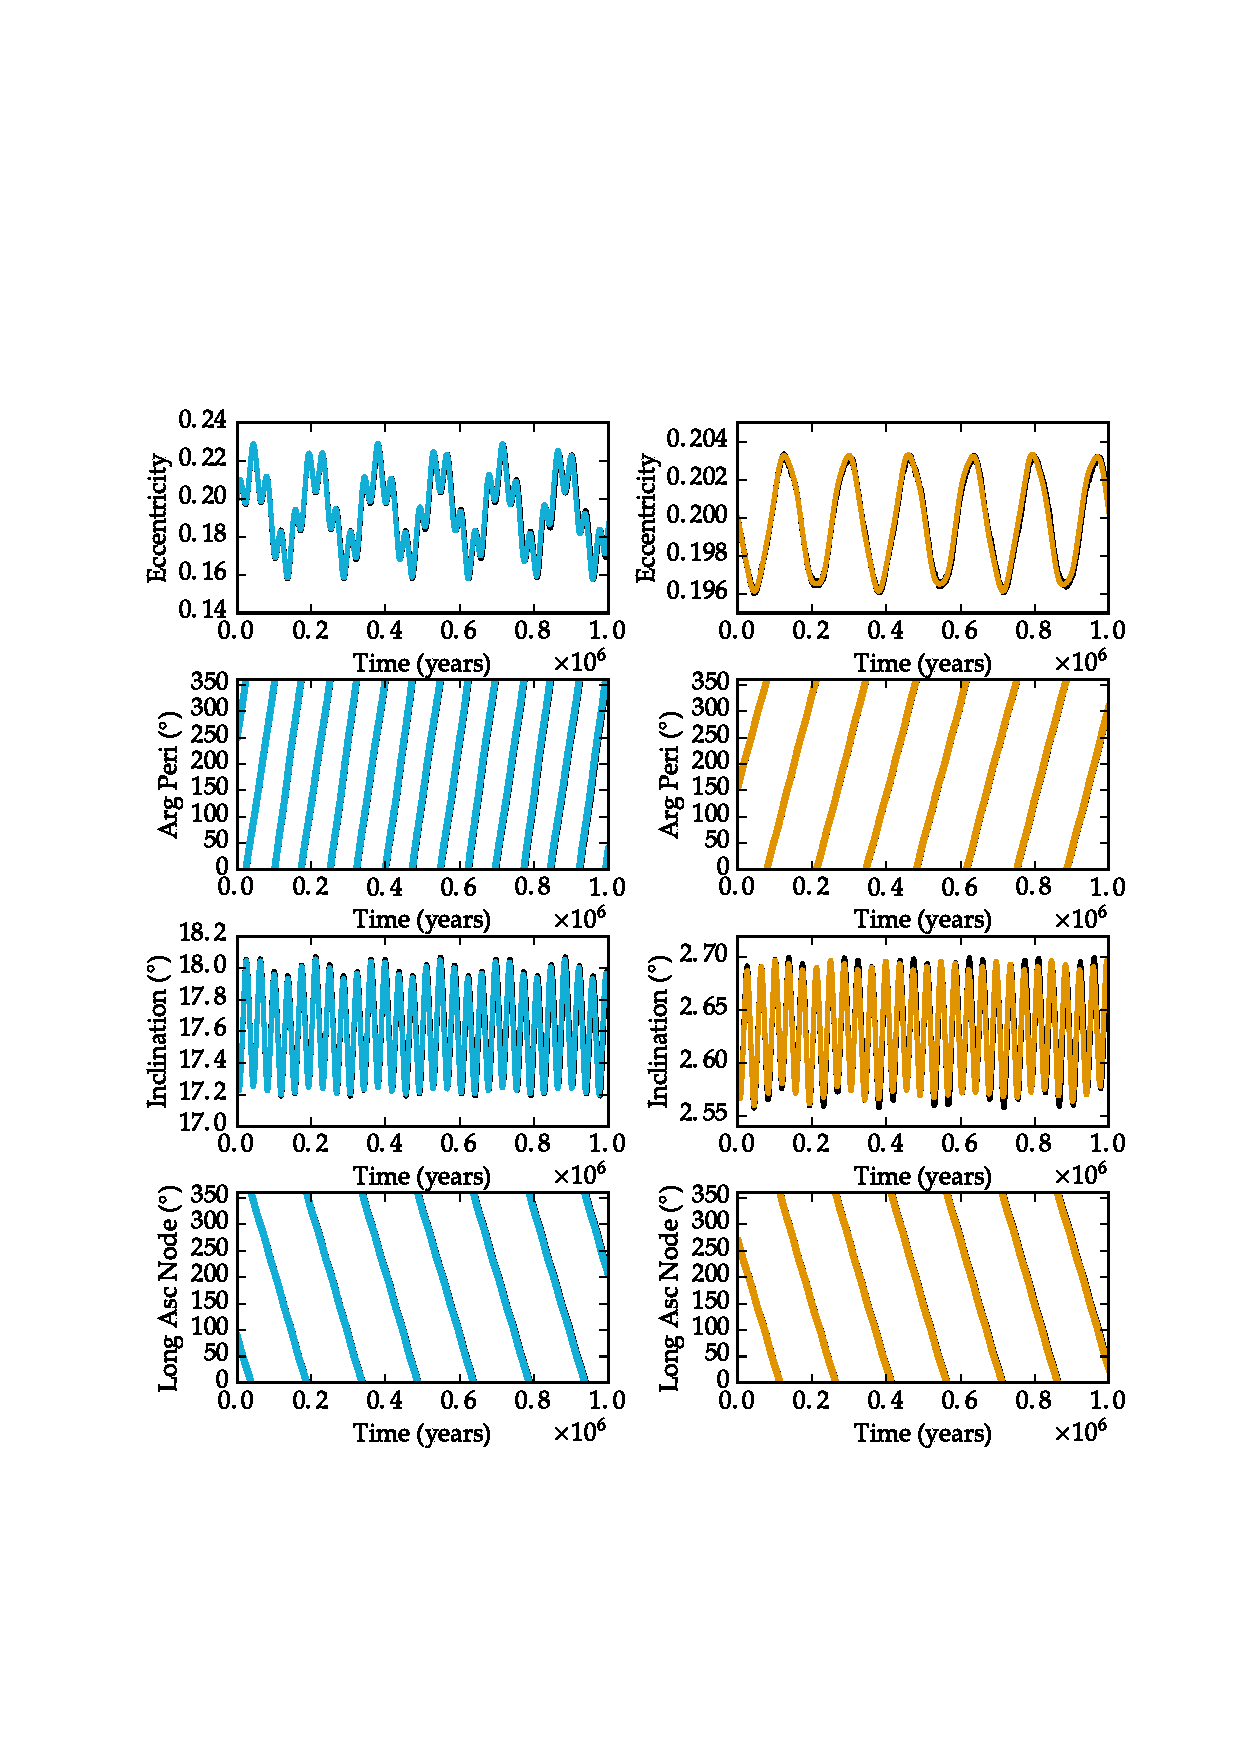
\includegraphics[width=\textwidth]{orbcomp_mid_e_i.pdf}
\caption{Comparison between the \distorb module and the N-body code and 
   {\footnotesize \texttt{HNBody}} for one of our 2
   planet test cases. Planet b is represented on the left, putative
   planet c on the right. {\footnotesize \texttt{HNBody}} evolution is in 
   black, \distorb in blue for planet b, orange for planet c.}
\label{fig:orbitvalid}
\end{figure} 

\subsection{Rotational Evolution from Orbits and the Stellar Torque: \distrot}
\label{sec:models:distrot}
% Russell
Our obliquity model, \distrot (for ``disturbing function rotation
evolution''), uses the equations of motion developed in
\cite{Kinoshita1975, Kinoshita1977} and utilized in numerous studies 
including  \cite{Laskar1986,Laskar1993a,Laskar1993b}, and \cite{Armstrong14}.  
It treats the planet as an oblate spheroid (having an axisymmetric equatorial
bulge), with a shape controlled by the rotation rate (see below). The planet then is
subject to a torque from the host star, which causes axial precession,
and changes in its orbital plane due to perturbations from a companion
planet, which directly change the obliquity angle.  This model is thus
dependent on \distorb through the eccentricity, the inclination, the 
longitude of ascending node $(\Omega)$, and the derivatives $dp/dt,
dq/dt$ (Eqs.~\ref{eqnp} and \ref{eqnq}).

The equations for obliquity and precession angle $(d\psi/dt,
dp_A/dt)$, also contain a singularity at $\psi = 0$, so we transform
to the variables:
\begin{align}
\xi & = \sin{\psi} \sin{p_A} \\
\zeta & = \sin{\psi} \cos{p_A} \\
\chi & = \cos{\psi}.
\end{align}
The third variable, $\chi$ is necessary to preserve domain information. Hence,
we ultimately have three variables to integrate rather than two, however, the
addition of a third variable/equation does not produce appreciable slow down.

Since we couple obliquity evolution in \distrot to tidal evolution in \eqtide, it is 
necessary to account for changes in the planet's shape (its dynamical ellipticity)
as its rotation rate changes due to tides. Following the examples of 
\cite{Atobe2007, Brasser2014}, we scale the planet's oblateness coefficient, $J_2$ 
(from which the dynamical ellipticity, $E_d$, can be derived), with the radius $R_p$, 
rotation rate $\omega_{rot}$, and mass $M$, as:
\begin{equation}
J_2 \propto \frac{\omega_{rot}^2 R_p^3}{M}.
\end{equation}
We use the Earth's $J_2$ as a proportionality factor. As pointed out by 
\cite{Brasser2014}, around a rotation period of 13 days, $J_2$ calculated in this 
way reaches the $J_2$ of Venus, which maintains this shape at a much slower 
rotation speed, and so, following their example, we set the 
minimum $J_2$ value to the  $J_2$ of Venus.
 
In the presence of strong tidal effects, as we would expect at Proxima b's orbital 
distance, the obliquity damps extremely quickly (in a few hundred kyr). Because 
of this, we do not expect this planet to have significant obliquity variations. Our 
purpose for including this model in our study is to look for Cassini states 
\citep{Colombo1966}---in the presence of strong tidal effects and perturbations
from companion planets, the planet's obliquity damps to some non-zero value, 
as we observe for Mercury and a number of solar system satellites, including 
Earth's moon. To quantify the existence of Cassini states, we use the formula:
\begin{equation}
\sin{\Psi} = \frac{(\hat{k}\times \hat{n}) \times (\hat{s} \times \hat{n})}{ | \hat{k}
\times \hat{n}  | \left | \hat{s} \times \hat{n} \right |},
\label{eqn:cassini}
\end{equation}
where $\hat{k}$, $\hat{s}$, and $\hat{n}$ are unit vectors associated with 
the total angular momentum of the planetary system, the spin of the planet,
and the planet's own orbital angular momentum \citep[see][]{Hamilton2004}.
In a Cassini state, the three vectors will be approximately constrained to a
single plane and the angle $\Psi$ will oscillate (with small amplitude) 
about $0^{\circ}$ or $180^{\circ}$, so $\sin{\Psi}$ will approach zero. 
We will refer to $\sin{\Psi}$ as the ``Cassini parameter''.

\subsection{Radiogenic Heating: \radheat}
\label{sec:models:radheat}

The first of two geophysical modules tracks the adundances of
radioactive elements in the planet's core, mantle and surface. We
consider 5 radioactive species: $^{26}$Al, $^{40}$K, $^{232}$Th,
$^{235}$U, and $^{238}$U. These elements have measured half-lifes of
$7.17 \times 10^5$, $1.251 \times 10^9$, $1.405 \times 10^{10}$,
$7.038 \times 10^8$, and $4.468 \times 10^9$ years, respectively. The
energy associated with each decay is $6.415 \times 10^{-13}$,
$2.134 \times 10^{-13}$, $6.834 \times 10^{-12}$,
$6.555 \times 10^{-12}$ and $8.283 \times 10^{-12}$ J, respectively.

We will consider 4 different abundance ratios. First, we consider an
Earth-like case with standard abundance concentrations
\citep[\eg][]{Korenaga03,Arevalo09,Huang13}. Note that geoneutrino
experiments are able to measure the decay products of $^{232}$Th and
$^{238}$U \citep{Raghavan98,Araki05,Dye10}.

The second case use chondritic abundances, in which we augment the
mantle's $^{40}$K budget by a factor of 30 in number to match the
potassium abundance seen in chondritic meteorites
\citep{AndersGrevesse89,Arevalo09}. Such high potassium abundances could be
present if the planet formed beyond the snowline where potassium, a
volatile, is more likely to become embedded in solids.

The third case is a planet containing 1 part per trillion (ppt) of
$^{26}$Al initially. If the planet formed within 1 Myr, either by
planetesimal accumulation or a direct collapse in the outer regions of
Proxima's protoplanetary disk, then not all the $^{26}$Al would have
decayed. A planet that formed quickly would likely have more than 1
ppt of $^{26}$Al, but as we will see in $\S$~\ref{sec:results}, our
geophysical module \thermint cannot handle heating rates much in
excess of this abundance. \xxx{How does this compare to Earth's 
initial budget of 26Al?}

The final case is an inert planet with no radioactive particles. This
case is very unlikely in reality, but serves as a useful end-member
case to bound the evolution of Proxima b.

\subsection{Geophyiscal Evolution: \thermint}
\label{sec:models:thermint}

We model the coupled core/mantle evolution of Proxima b with a
1-dimensional model that has been tuned to reproduce Earth
\citep{DriscollOlson11,DriscollBercovici13,DriscollBercovici14,DriscollBarnes15}, and the
reader is referred to those studies for a comprehensive description of
it. Briefly, the model is based on tracking the core and mantle
temperatures, and the rest of the geophysics depends on them. The code
includes heat transport through the core/mantle boundary (CMB) for
both convective and non-convective cores, melt production and eruption
from the mantle, latent heat produced by mantle solidification and,
when applicable, tidal heating, see $\S$~\ref{sec:models:eqtide}. Magnetic field
generation is assumed to result from convective motion in the core,
and the magnetic moment and magnetopause radius are trivially
calculated from the temperature difference between the core and
mantle, as well as from the pressure of the stellar wind at the orbit
of Proxima b.

Our model has been validated by simultaneously and self-consistently
reproducing the modern Earth's surface energy flux, magnetic
properties, eruption fluxes, plate speeds, and outgassing rates. It
has also been used to successfully reproduce the divergent evolution
of Venus and Earth under the assumption that they formed without
atmospheres, and very similar compositions and temperatures
\citep{DriscollBercovici13}. This reproduction does require the tuning of
numerous free parameters, but all choices are reasonable, especially
in light of the poor information available on Venus' interior. While
this model is generic in many ways, it does have its limits in that it is
explicitly designed for an Earth-like composition, structure, mass and
radius. However, the minimum mass for Proxima b is negligibly far from
Earth as far as this model is concerned. Further, \thermint cannot
handle initial mantle temperature below $\sim$1500~K, at which point
diffentiation would not occur, or above 8000~K, where non-linear
rheologies require different assumptions and equations.

The \thermint modules can be directly coupled to \eqtide as shown in
\citep{DriscollBarnes15}. In that case, we assume all the tidal power
is deposited in the mantle and the heating changes the viscocisty, and
in turn the tidal $Q$. \cite{DriscollBarnes15} used a visco-elastic
model in which the tidal heating is a maximum for mantle temperature
near 1800~K, and thus cooling planets pass through a maximum in
temperature.

\subsection{Galactic Effects: \galhabit}
\label{sec:models:galhabit}
% Russell/Tom
Prox Cen is tenuously bound, if it is gravitationally bound at all, to 
the binary $\alpha$ Cen A and B. Because of this, it is worthwhile
to investigate the effects of the galactic environment on 
Prox Cen's orbit. We model the changes produced by galactic tides 
and stellar encounters using the equations and prescriptions 
developed by \cite{Heisler1986, Heisler1987, Rickman2008} 
for the Oort cloud (Prox Cen is arguably a high mass Oort cloud 
object, for $\alpha$ Cen A and B). We utilize an updated galactic 
density of $\rho_0 = 0.102~\msun \rm{pc}^{-3}$ \citep{Holmberg2000} and treat 
$\alpha$ Cen A and B as a single point mass with $M = 2.1$ 
M$_{\odot}$ (with the recently updated masses given by 
\cite{PourbaixBoffin16}). This is a somewhat crude approach, as 
the two stars produce a significant quadrupole moment associated 
with their orbits---a back-of-the-envelope calculation indicates
that the torque associated with this quadrupole potential would 
be equal to the galactic tidal torque at $\sim 2000$ au. Hence, 
the effect of the binary host should be minor though still important 
at Prox Cen's estimated distance of $~15,000$ au, especially if 
the star has significant eccentricity. However, the modeling of the 
triple system in a comprehensive way is sufficiently complicated
\citep[see, i.e.][]{Harrington1968, Ford2000} to place it beyond 
the scope of this work. Instead, we restrict ourselves to the 
secular effects of galactic tides and passing stars 
and will revisit the triple star dynamics in a future work. 

If Prox Cen is gravitationally bound, galactic tides and stellar 
encounters can pump its eccentricity to values large enough to 
cause disruption from the system, and/or a periastron distance 
so close to the binary $\alpha$ Cen that we would expect 
consequences for any planetary system, such as eccentricity 
excitation. In such situations, Proxima b may have significant tidal 
heating despite the circularization time scale. 

Following \cite{Heisler1987,Rickman2008}, we model stellar
encounters in a stochastic Monte Carlo approach, estimating times 
of encounters from the stellar density and velocity dispersion, 
and then randomly drawing stellar magnitudes, and velocities 
from the distributions published in \cite{Garciasanchez2001}. 
The impact parameter is calculated from the relative 
velocities (stellar velocity relative to the solar apex velocity, 
\cite[see][]{Rickman2008}), and then a $\Delta v$ is applied to
Proxima's orbit according to the impulse approximation
\citep{Remy1985}. The masses of passing stars are calculated 
using the empirical relations from \cite{Reid2002}.

As previously noted, the metallicities of $\alpha$ Cen A and B 
suggest that the system formed at a galactocentric distance of 
$\lesssim 4.5$ kpc \citep{Loebman16}. To model the potential 
effects of radial migration on the triple star system (again, 
assuming Proxima is gravitationally bound to A and B), we 
scale the total mass density and stellar density of the galaxy 
according to the radial scale lengths ($R_{\star}, R_{gas}$) found
by \cite{Kordopatis15}. The dark matter density at each distance 
is estimated from their spheroidal model---unlike the disk models 
used for stars and gas, this model is not axisymmetric, however, 
as the dark matter near the mid plane of the disk makes up 
$\lesssim 1\%$ of the total density, it is a decent approximation 
to assume axisymmetry of the total mass density, as the 
\cite{Heisler1986} tidal model assumes. We scale the velocity 
dispersions of the nearby stars as a decaying exponential 
with twice the stellar scale length, $2R_{\star}$, multiplied by 
$\sqrt{t}$, where $t$ is the time since galactic formation, as found 
to be broadly true in galactic simulations 
\citep{Minchev2012, Roskar2012}. In this fashion, the velocity 
dispersion grows slowly in time at all galactic radii and it grows 
larger closer to the galactic center.
The apex velocity, \ie the velocity of the star with respect to
the Local Standard of Rest, will vary according to the detailed
orbital motion
of Proxima through the galaxy, including the radial migration.  For the
purposes of this study, we
simply leave the apex velocity a constant, assuming the current Solar
value is typical, and we will revisit this problem in a later study.

With such scaling laws in place, we model radial migration 
as a single, abrupt jump in the galactocentric distance of the 
system. The reasoning behind this approximation is that N-Body 
simulations show migration to occur generally over the 
course of a single galactic orbit \cite{Roskar2010}, hence the 
migration time is short compared to the age of the stellar system.
We then randomly choose formation distances over the range 
$(1.5,4.5)$ kpc and migration times over the range $(1,5)$ Gyr 
since formation.

\subsection{The Coupled Model: \vplanet}
\label{sec:models:vplanet}
% Rory
The previous modules are combined into a single software program
called \vplanet. This code is written in C and is designed to be
modular so that for any given body, only specific modules are applied
and specific parameters integrated in the forward time direction. 
Parameters are integrated
using a 4th order Runge-Kutta scheme with a timestep equal to $\eta$
times the shortest timescale for all active parameters, \ie
$x/(dx/dt)$, where $x$ is a parameter. In general, we obtain convergence if
$\eta~\le~0.01$. A more complete and quantitative description of
\vplanet~will be presented soon (Barnes et al., in prep.). 

\xxx{dflemin3: Here, a brief reference to how a model is given model is calibrated/validated
could help to assuage a read/reviewer.  For example, you could say that THERMINT is calibrated
to the earth an discussed in the already peer-reviewed/published Driscoll and Barnes 2015.  I'm a bit 
worried people will call BS on model coupling (even though our results are rock-solid in my mind), so
a simple reference here in addition to everything in the module sections would help.  I guess this is hard because
no one has ever attempted a crazy thing like VPLANET, but taking an extra step to show that VPLANET is robust
and rigorous will go a long way since the actual VPLANET presentation paper is months away.}

\xxx{rd: We validated vplanet using the recently released planetary model, \texttt{No Man's Sky}}

Each individual model is validated against observations in our Solar
System or in stellar systems. When possible, conserved quantities are
also tracked and \xxx{required to maintain in acceptable limits}. \xxx{While a
validation against a single system or uniform data set, not such
observation exists for a full \vplanet~simulation. (what?)} Matching
simulations to systems like Proxima Centauri is likely the only way to
\xxx{convincingly} validate the code.

\section{Results\label{sec:results}}
% All

\subsection{Galactic Evolution}
\label{sec:results:galactic}
% Russell
The high abundance of heavy elements measured for the $\alpha$ Cen 
A and B stars ([Fe/H] $\sim 0.3$) is difficult to explain without radial 
migration \citep{Kordopatis15,Loebman16}. Hence there is a high likelihood 
these stars formed at a galactic distance $R\lesssim 4.5$ kpc. Prox Cen's [Fe/H] 
has been inferred from its' association with $\alpha$ Cen \citep{Johnson2009},
however, it is not entirely clear that that the star is gravitationally bound to 
$\alpha$ Cen \citep{MatvienkoOrlov14} or that it must have formed alongside 
$\alpha$ Cen. Nevertheless, we assume for this study that Prox Cen formed in 
the same environment as $\alpha$ Cen and is either still gravitationally bound or
has recently come unbound from the inner binary, and model the effects of 
galactic tides and stellar encounters, assuming initial orbits that allow for 
Prox Cen to be at roughly its current distance from $\alpha$ Cen.

We have run two experiments to explore the effects of radial migration: the first, 
set \textbf{A} places the system in the solar neighborhood, randomly selecting 
orbital parameters broadly consistent with the observed positions, for 10,000 
trials. In set \textbf{B}, we have taken the same initial conditions and randomly 
selected formation distances over the range (1.5,4.5) kpc and migration times
over (1,5) Gyr after formation, after which the system is moved to the solar 
neighborhood (8 kpc). 

Simulations were halted whenever Prox Cen's orbit passed within 40 au of 
the center of mass of $\alpha$ Cen A and B, when it passed beyond 1 pc,
or when it became gravitationally unbound ($e > 1$). In set \textbf{A} 
(see Figure \ref{fig:galacdist}, left-hand panels), 1506 
out of 10,000 simulations were halted because of one of the three above conditions.
Closer inspection reveals that the majority of these (1289) were halted because 
Prox Cen's periastron passed within 40 au of $\alpha$ Cen. Of those that didn't
halt, another 1363 passed within 200 au and 620 passed within 100 au. Including 
those trials that were halted for any reason, 2688 ($27\%$) passed within 200 au and
1929 ($19\%$) passed within 100 au. 

The importance of this is that $\sim 100$ au is the distance a close encounter with a 
$\sim 2 M_{\odot}$ star would disrupt a planetary system similar to the solar system
\citep{Kaib13}. The fact that $\alpha$ Cen is a binary itself, with a large eccentricity 
($e \sim 0.5$) probably increases the disruption distance still further.
Of course, Prox Cen is very different from the sun and may never 
have formed a planetary system like the one we inhabit (with gas giants at large 
orbital distances), however, it may still have had an extended planetary system
at some point. If that is the case, the system may have been disrupted, or may be
disrupted in the future, by a close periastron passage with $\alpha$ Cen.

Radial migration makes close passages and disruption more likely. The right 
panels in Figure \ref{fig:galacdist} compare the trials that survived 7 Gyr (to completely 
capture the range of possible ages of \acen)
and those that were halted (disrupted) due to the previously mention conditions 
for set \textbf{B}. In this set, 2544 trials were halted and 1717 of those were 
due to periastron reaching below 40 au. Of the remaining cases, 1333 had 
periastron distances $< 200$ au and 634 below $<100$ au. Including
cases that were halted, 3195 ($32\%$) passed within 200 au and 2452 ($25\%$) 
passed within 100 au.

\begin{figure}
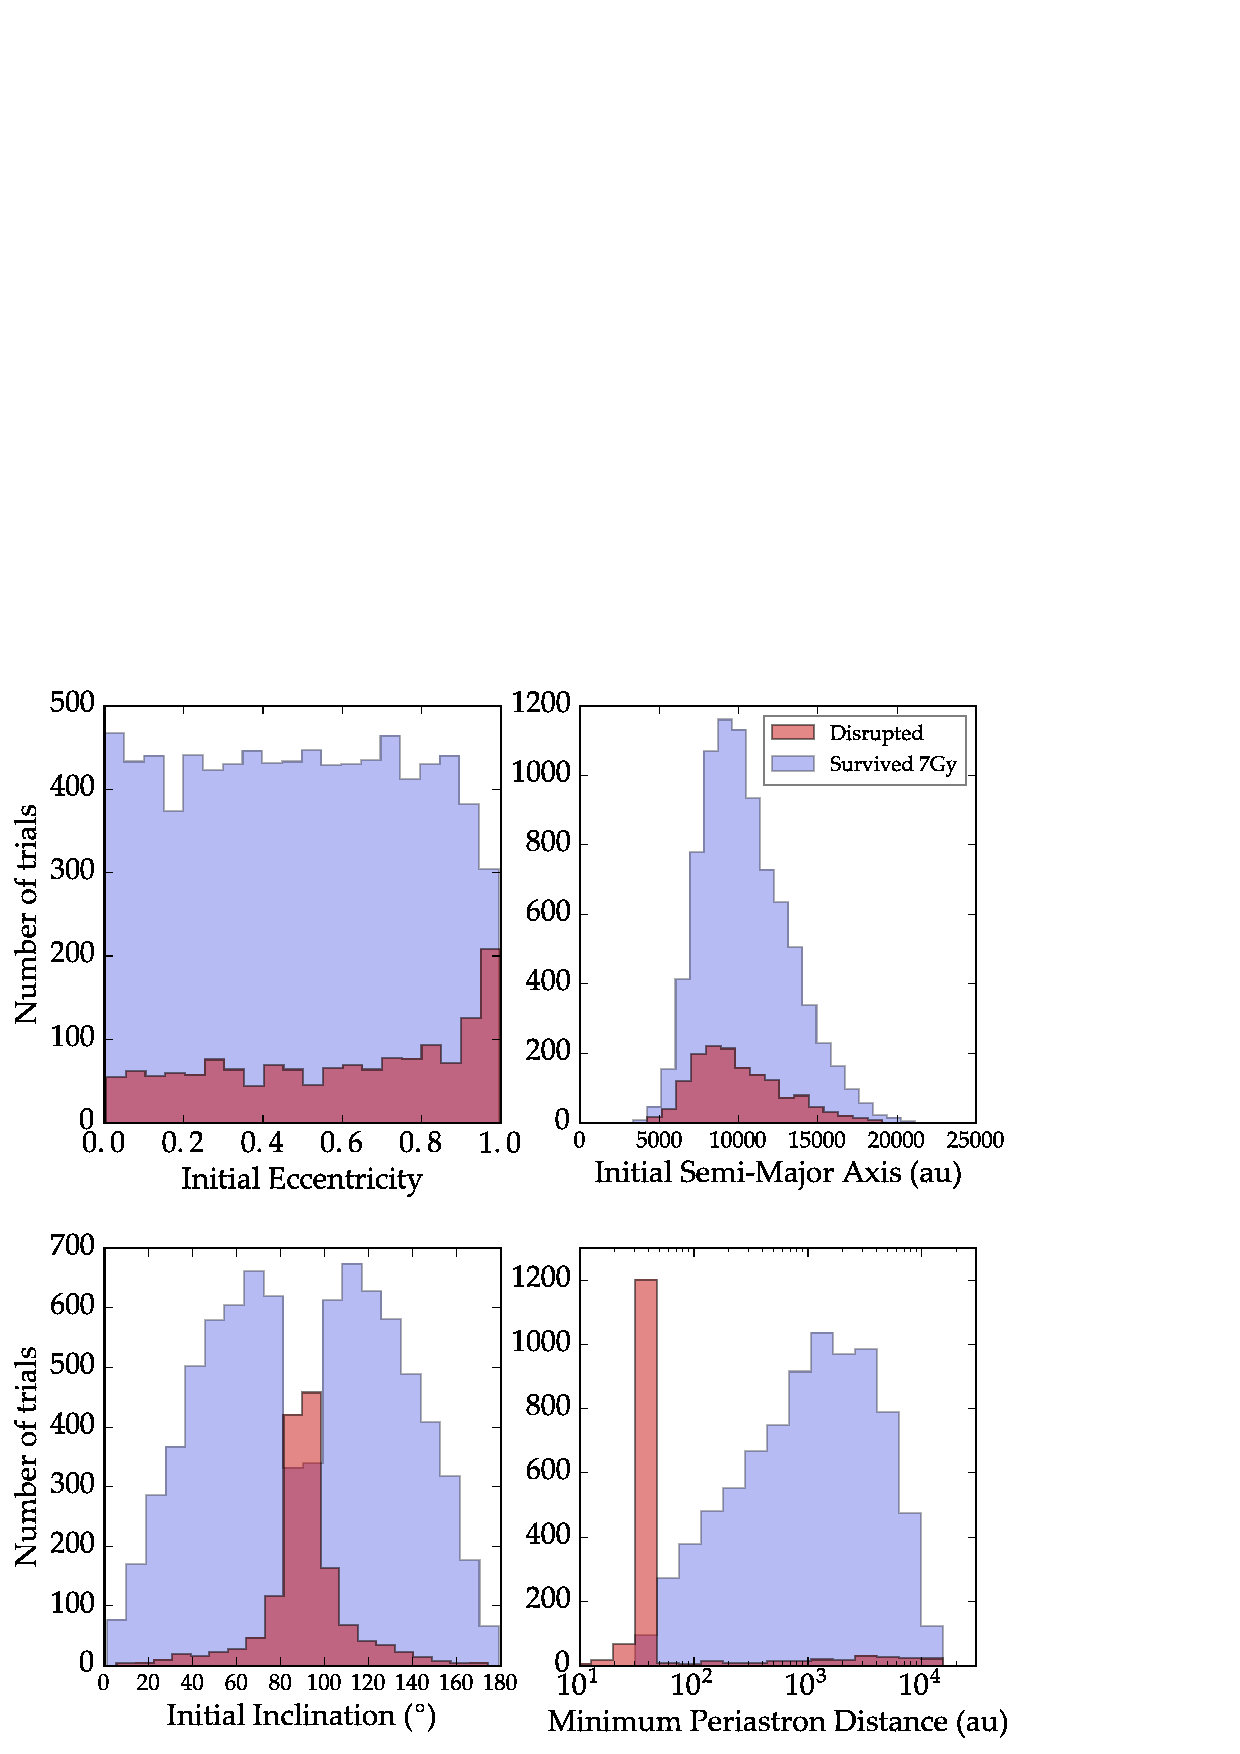
\includegraphics[width=0.5\textwidth]{nomigrdist.pdf}
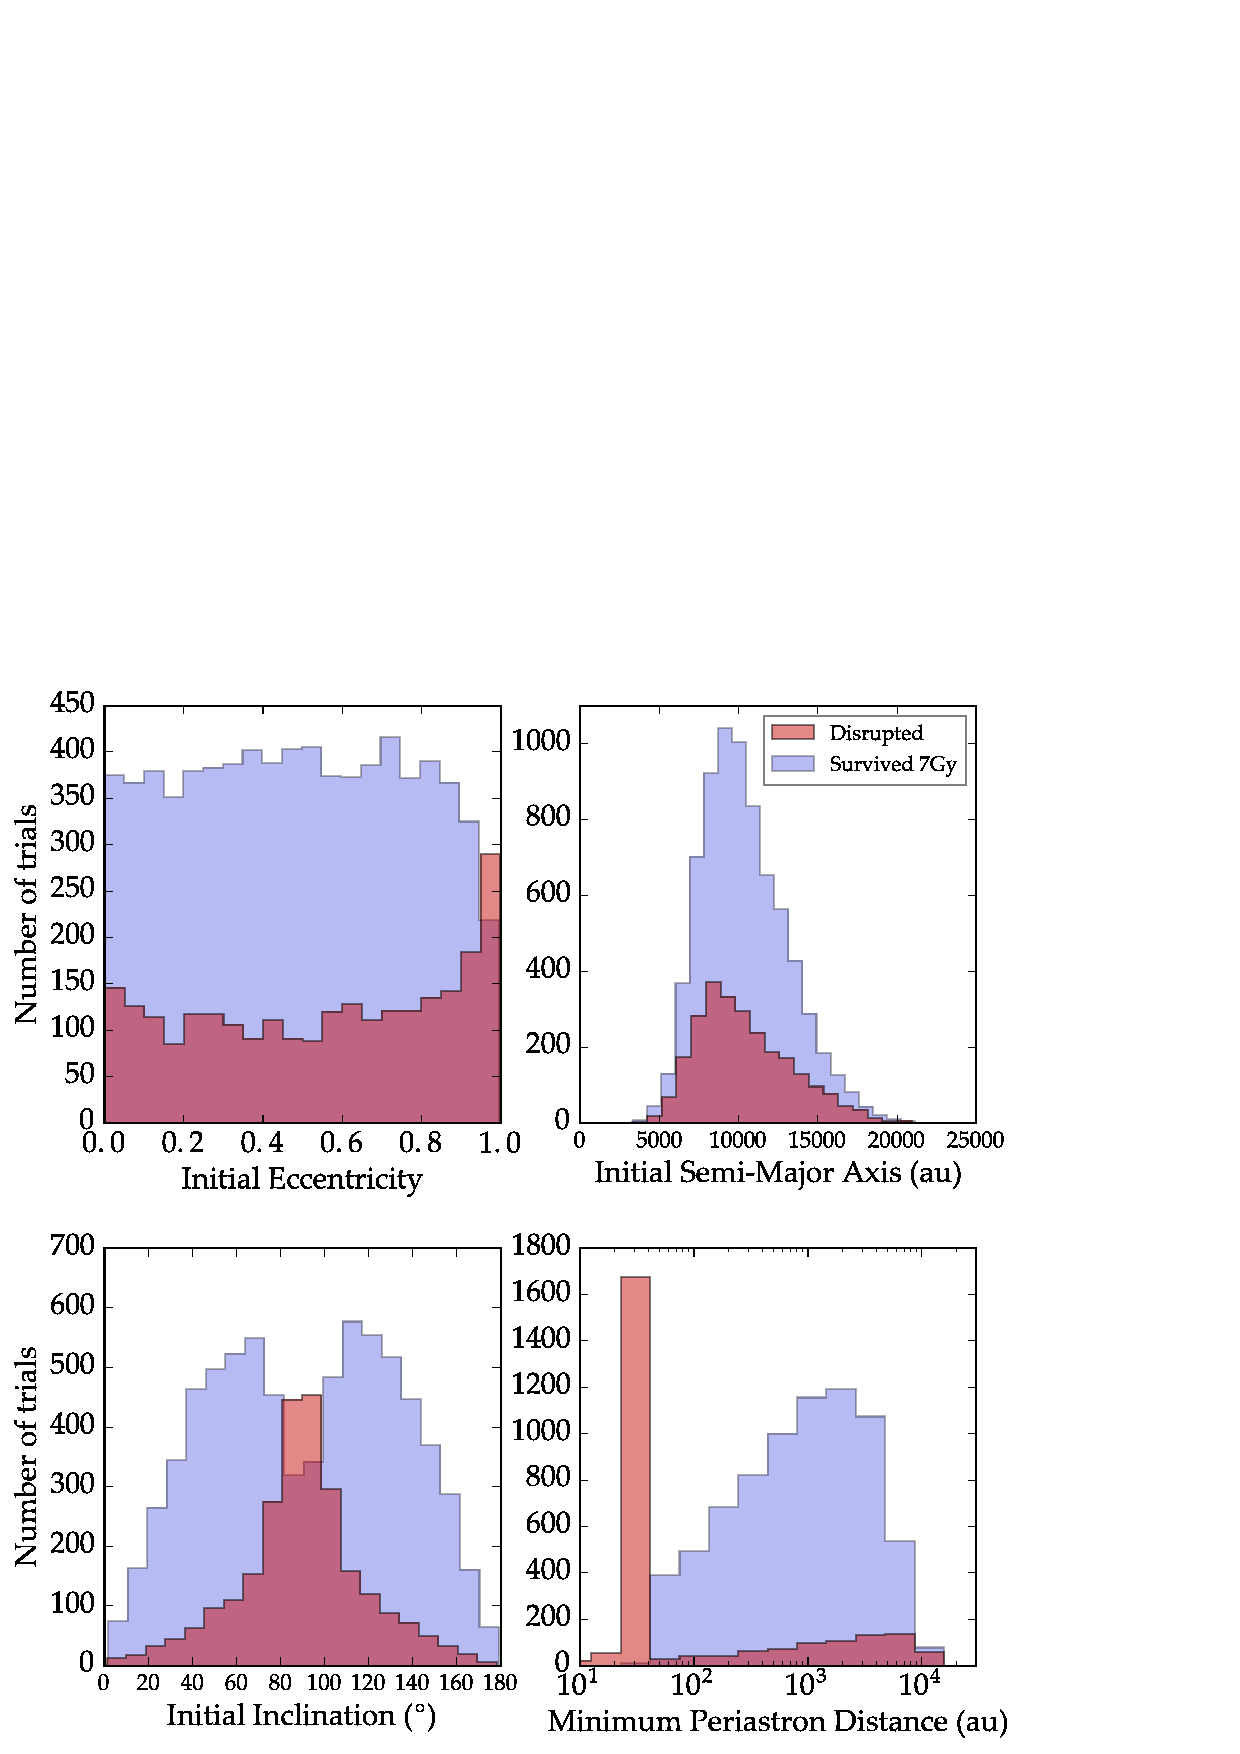
\includegraphics[width=0.5\textwidth]{migrdist.pdf}
\caption{Distributions of trials in which Prox Cen's orbit about $\alpha$ Cen
  is disrupted (red) and trials in which it survives to $>$ the age of the 
  system (blue). Set {A} (no migration) is on the left and set {B} (with 
  radial migration) is on the right. Each half of the figure shows the 
  distributions as a function of initial eccentricity (upper left), initial 
  semi-major axis (upper right), initial inclination relative to the galactic 
  disk (lower left), and the minimum periastron distance over the entire 
  simulation (lower right). Generally, eccentricity and inclination are the 
  greatest determinants of stability, with high $e$ and $i \sim 90^{\circ}$ 
  (i.e. low $\hat{Z}$-angular momentum) cases being the least stable. 
  Systems which formed interior to 4.5 kpc from the galactic center 
  (set \textbf{B}, right half of figure) are disrupted more frequently than 
  those which were placed in the solar neighborhood from the beginning. 
  Amongst the cases we considered ``stable'', a significant fraction still 
  have Prox Cen pass within a few hundred au of $\alpha$ Cen A and B.}
\label{fig:galacdist}
\end{figure}


% Fig. 1: Sample R_gal vs. time
% Fig. 2: Encounter frequency vs. R_gal
\begin{figure}
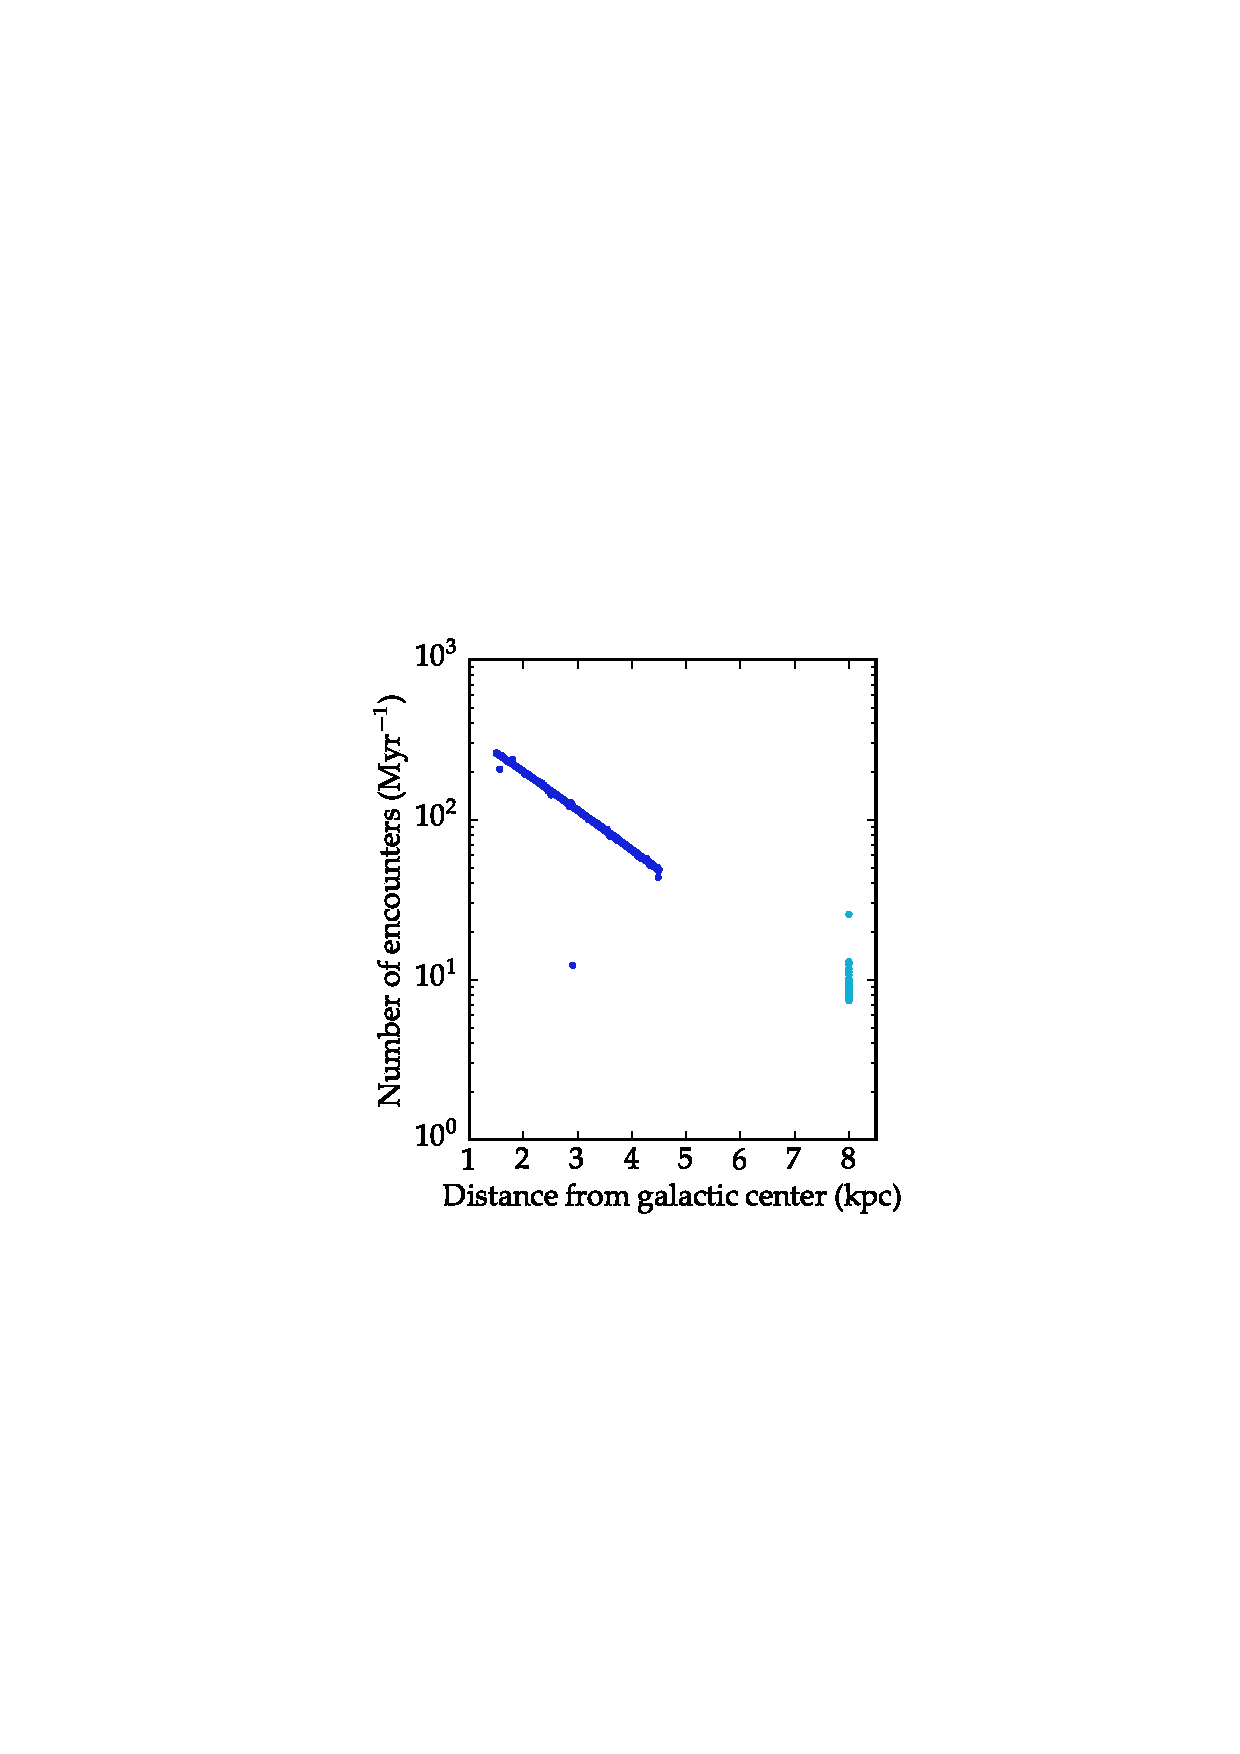
\includegraphics[width=0.5\textwidth]{encvsR.pdf}
\caption{Stellar encounter rates as a function of galactocentric distance.
  Dark blue points correspond to pre-migration encounter rates, light 
  blue to post-migration. The large outlier in the light blue, 
  solar-neighborhood, is due to small number statistics---the system 
  in that simulation was disrupted shortly after migration. There is some 
  scatter in the solar-neighborhood points because of the time dependence 
  of the stellar velocity dispersion. At the tail end of the simulations, we 
  match the encounter frequency of 10.5 Myr$^{-1}$ from previous 
  studies \citep{Garciasanchez2001,Rickman2008}.}
\label{fig:encrates}
\end{figure}

% Fig. 3: Sample evolution of Prox's orbit: a) semi, peri, apo, b) incl

\begin{figure}
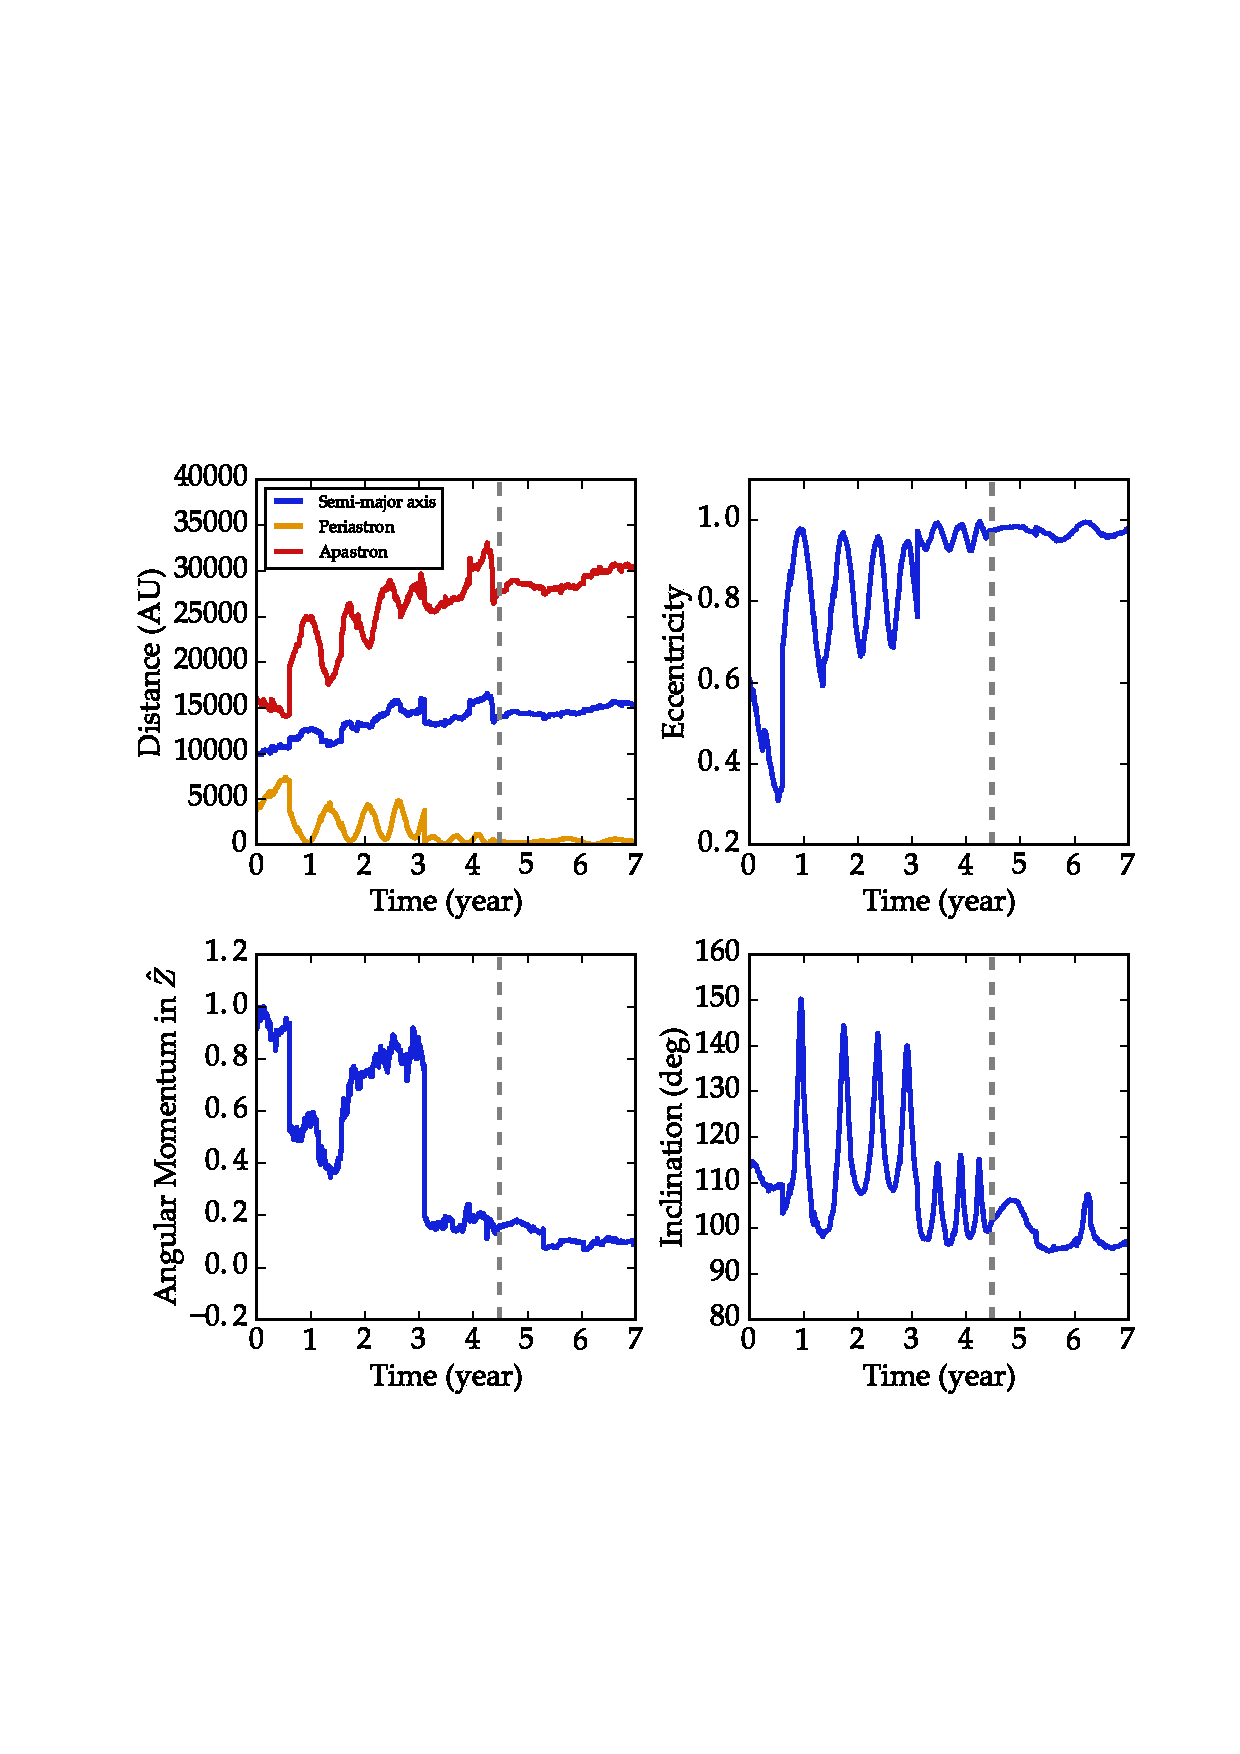
\includegraphics[width=\textwidth]{evol_Vpl_0257.pdf}
\caption{An example of the orbital evolution of Prox Cen in the galactic 
  simulations. The upper left panel shows the semi-major axis, periastron 
  distance, and apastron distance, the upper right shows the eccentricity, 
  the lower left shows the angular momentum in the $\hat{Z}-$direction, 
  and the lower right shows the inclination with respect to planet of the 
  galactic disk. The system was given a formation distance of $R = 3.78$ 
  kpc and the vertical dashed line shows the time of migration (to 8 kpc). 
  The angular momentum in $\hat{Z}$ (the action $J_z$) is unchanged by 
  galactic tides---eccentricity and inclination exchange angular momentum 
  in such a way that this quantity is conserved---thus its evolution is purely 
  due to stellar encounters. In this particular case, the eccentricity of Prox Cen 
  grows such that its periastron dips within 50 au of $\alpha$ Cen A and B.}
\label{fig:galevolution}
\end{figure}

One potential issue with our orbit-averaged approach is that for Prox Cen in the 
semi-major axis range ($\sim5000$ to $\sim20000$) au, the orbital periods 
span a range of 240 thousand to 2 million years. Thus it may be possible in 
the simulations for Prox Cen's periastron to come very close to $\alpha$ Cen 
for a short period of time and then evolve to a larger distance before Prox Cen 
ever \emph{actually reaches} periastron. Hence, we are potentially halting 
simulations in which 
Prox Cen may not actually pass within 40 au of $\alpha$ Cen. Our results 
should thus be seen as an upper limit on the number of configurations 
that lead to close encounters between Prox Cen and $\alpha$ Cen.
 
\subsection{Orbital/Rotational/Tidal Evolution}
\label{sec:results:orbital}
% Russell/Rory/Diego?

\xxx{dflemin3: For the orbital/rotatinonal end cases, I would find brief habitability comments to be useful.  For example,
if some high eccentricity is maintained -> more tidal heating or something of that nature.  Also, how does being in a certain
Cassinni state impact habitability, surface water content, does it at all?  Little allusions back to how these things impact
habitability could be useful as it will help to continue to hammer the VPLANET mission of modeling how all these things
impact ultimate goal of modelling habitability.}

We begin exploring the dynamical properties of the orbits and spins by
considering the tidal evolution of planet b if it is in isolation. In
this case, we need only apply \eqtide~to both Proxima and b and track
$a, e, P_{rot},$ and $\psi$. We find that if planet b has $Q~=~12$ \xxx{justify this choice?},
then an initially Earth-like rotation state becomes tidally locked in
$\sim~10^4$ years, so it seems likely that if b formed near its
current location, then it formed in a tidally locked state and with
negligible obliquity.

Unlike the rotational angular momentum, the orbit can evolve on long
timescales. In the top two panels of Fig.~\ref{fig:eqtide}, we
consider orbits that begin at $a~=~0.05$~AU and with different
eccentricities of 0.05 (dotted curves), 0.1 (solid curves) and 0.2
(dashed curves). In these cases $a$ and $e$ decrease and the amount of
inward migration depends on the initial eccentricity, which takes 2--3
Gyr to damp to $\sim~0.01$. For initial eccentricities larger than
$\sim~0.23$, the CPL model actually predicts eccentricity growth due
to angular momentum exchange between the star and planet
\citep{Barnes16}. This prediction is likely unphysical and due to the
low order of the CPL model, therefore we do not include evolutionary
tracks for high eccentricities.

The equilibrium tide model posits that the lost rotational and orbital
energy is transformed into frictional heating inside the planet. The
bottom panel of Fig.~\ref{fig:eqtide} shows the average surface energy
flux as a function of time. We address the geophysical implications of
this tidal heating in $\S$~\ref{sec:results:internal:tides}. Note that if planet
b begins with a rotation period of 1 day and an obliquity of
$23.5^\circ$, then the initial surface energy flux due to tidal
heating is $\sim~1$~kW/m$^{2}$.

\xxx{dflemin3: does this high surface flux desiccate the planet?  Brief comment on habitability could be useful here.}

\begin{figure} 
\begin{center}
\includegraphics[width=0.75\textwidth]{eqtide.ps}
\end{center}
\caption{Evolution of planet b's eccentricity (top), semi-major axis
  (middle), and tidal heating surface flux (bottom) assuming that
  initially $a~=~0.05$~AU and $e~=$~0.05 (dotted), 0.1 (solid) or 0.2
  (dashed). For reference the best fit semi-major axis and surface
  energy fluxes of Io and the modern Earth are shown by dashed black
  lines.}
\label{fig:eqtide}
\end{figure}

Next, we consider the role of additional planets, specifically the
putative planet with a 215 day orbit \citep{AngladaEscude16}. For
these runs we now add the \distorb and \distrot modules and track the
orbital elements of both planets, the spins of the star and planet b,
and the dynamical ellipticity of planet b. A comprehensive exploration
of parameter space is beyond the scope of this study, so we consider
two end-member cases: a nearly coplanar, nearly circular system, and a
system with high eccentricities and inclinations. The initial orbital
elements and rotational properties of the bodies are listed in Table \ref{tab:orbitic}.

\begin{table}[h]
\centering
\begin{tabular}{lccccccccc}
\hline\hline \\[-1.5ex]
& $m$ ($M_{\oplus}$)  & $a_s$ (au) & $a_l$ (au) & $e$ & $i$ ($^{\circ}$)
 & $\omega$ ($^{\circ}$) & $\Omega$ ($^{\circ}$) & $\psi$ ($^{\circ}$) & 
 $P_{rot}$ (days)\\[0.5ex]
\hline \\ [-1.5ex]
b & 1.27 & 0.0482817 & 0.05 & 0.001 & 0.001 & 248.87 & 20.68 & 23.5 & 1  \\
c & 3.13 & 0.346 & 0.346 & 0.001 & 0.001 & 336.71 & 20 & &  \\
\hline \\
b & 1.27 & 0.0482817 & 0.05 & 0.02 & 20 & 248.87 & 20.68 & 23.5 & 1  \\
c & 3.13 & 0.346 & 0.346 & 0.02 & 0.001 & 336.71 & 20 & &  \\
\end{tabular}
\caption{Initial conditions for Proxima 2-planet systems. The coplanar, 
  circular case is on top, the eccentric, inclined case below.}
\label{tab:orbitic}
\end{table}

In Fig.~\ref{fig:MultiLow} we show the orbital evolution for the low
$e$ and $i$ case over short (left) and long (right) timescales. As
expected, the planets exchange angular momentum, but over the first
million years there is no apparent drift to due tidal effects. On
longer timescales, however, we see the eccentricity of $b$ slowly decay
due to tidal heating. Note the differences in timescale for the decay
between Figs.~\ref{fig:eqtide} and \ref{fig:MultiLow}. The
perturbations from a hypothetical ``planet c'' maintain significant
eccentricities for long periods of time.

\begin{figure} 
\begin{center}
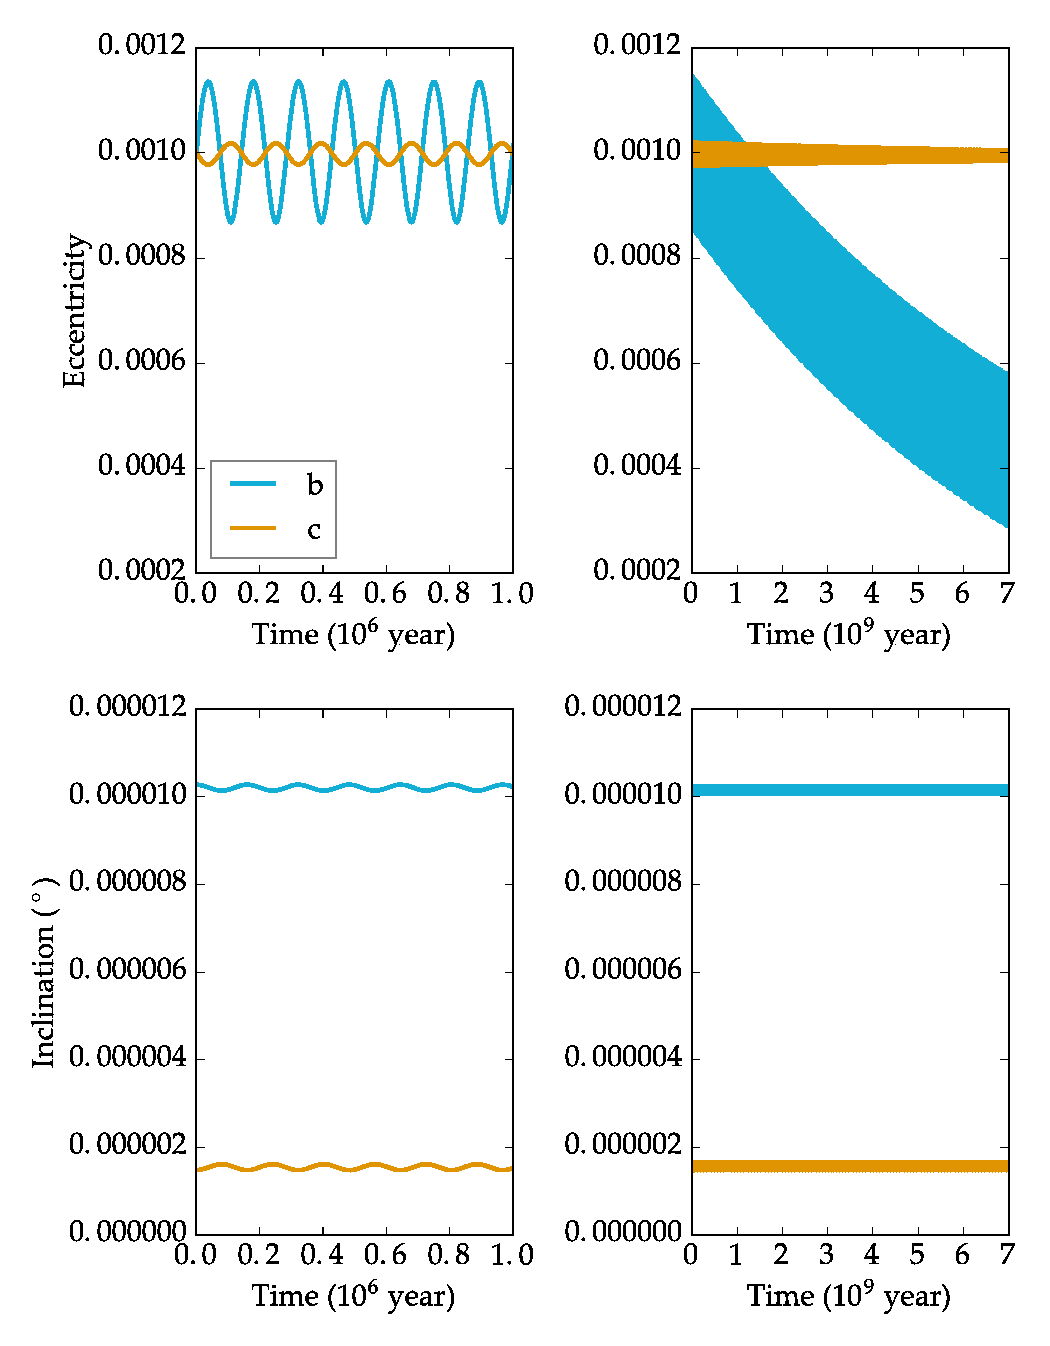
\includegraphics[width=0.75\textwidth]{MultiLow2.eps}
\end{center}
\caption{Evolution of orbital elements if a putative planet c exists with an 
orbital period of 215 days and both orbits are nearly circular and nearly 
coplanar. {\it Top Row:} Eccentricity. {\it Bottom Row:} Inclination.}
\label{fig:MultiLow}
\end{figure}

In Fig.~\ref{fig:MultiHigh}, we plot the orbital evolution for the
high $e$ and $i$ case. The eccentricity and inclination oscillations
are longer, and the eccentricity cycles show several frequencies due
to the activation of higher order terms in the coupling coupling of $e$ and
$i$. As in the low $e$ and $i$ case, the eccentricity damps more
slowly than in the unperturbed case. Note as well that the inclination
oscillation amplitude decays with time.

\begin{figure} 
\begin{center}
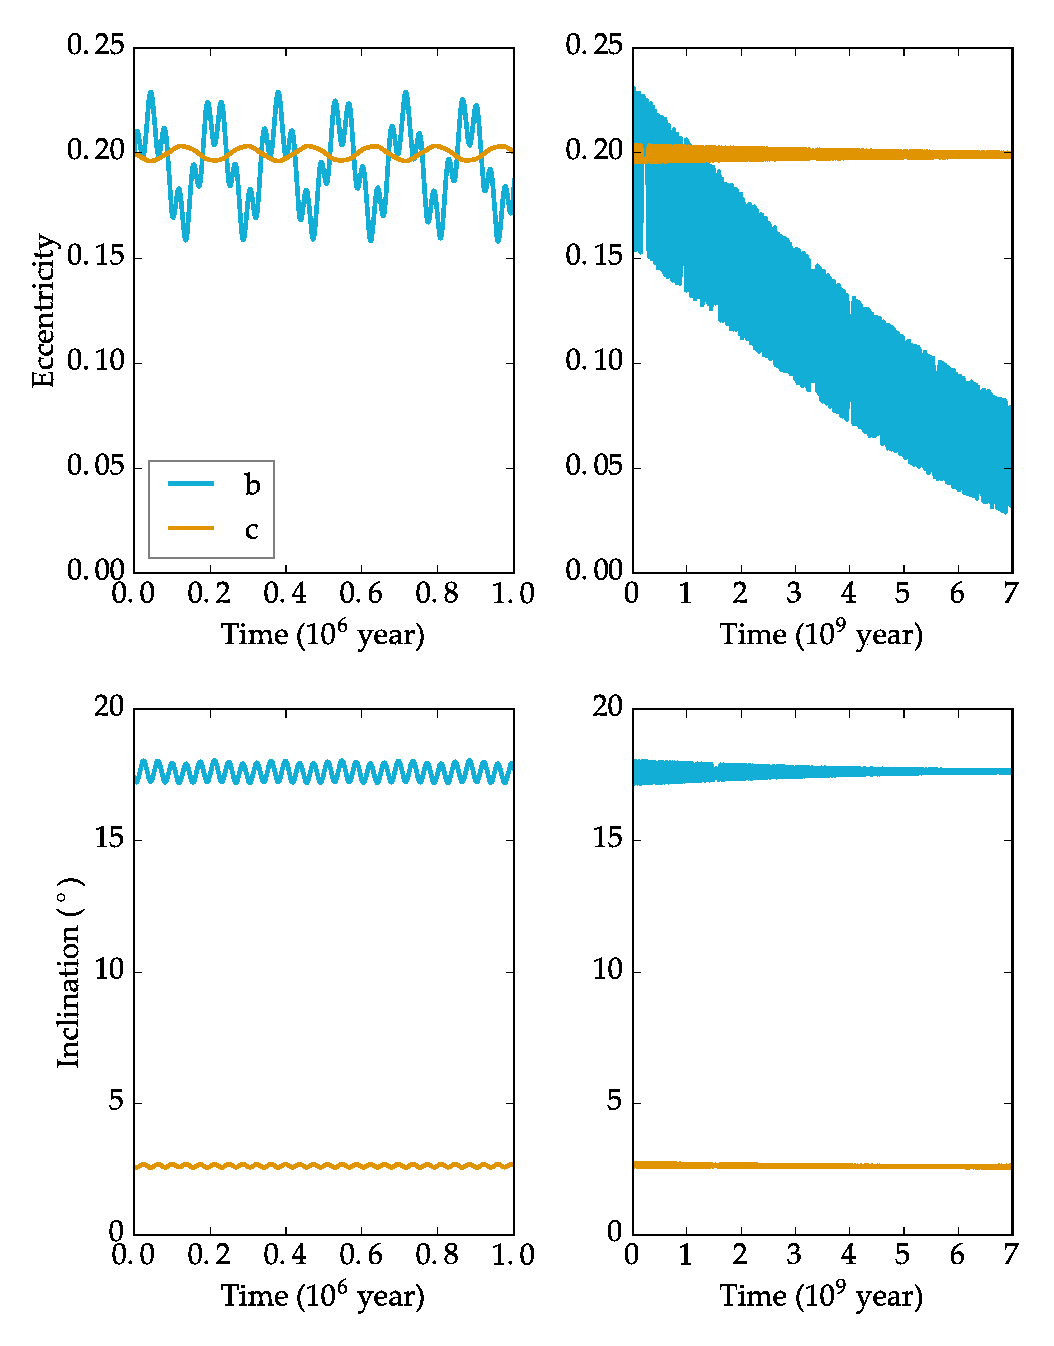
\includegraphics[width=0.75\textwidth]{MultiHigh2.eps}
\end{center}
\caption{Same as Fig.~\ref{fig:MultiLow}, but for the high $e,i$ case.}
\label{fig:MultiHigh}
\end{figure}

In Fig.~\ref{fig:MultiSpins}, we plot the evolution of the rotational
parameters for the two cases. In the top left panel, we show the
evolution of the rotational period. The rotation becomes tidally
locked very quickly (less than 1 Myr for all plausible values of $Q$
for an ocean-bearing world). 
In the high $e,i$ case, the planet briefly 
enters the 3:2 spin orbit resonance (like the planet Mercury).
The obliquity initially grows due to
conservation of angular momentum \citep{Correia08}, but then damps
down. For the high $e,i$ case, the obliquity reaches an equilibrium
value near $0.1^\circ$, while the low $e,i$ case drops all the way to
$10^{-8~\circ}$. The bottom left panel shows the evolution of the
dynamical ellipticity as predicted by the formulae from \cite{Atobe2007}.
The lower right panel shows the value of the Cassini Parameter 
(see Equation \ref{eqn:cassini}) for the two cases, both of
which becomes locked near 0, indicating the rotational and angular
momentum have evolved into a Cassini State, in this case it is Cassini
State 2, in which the spin and orbit vectors of planet b are on opposite 
sides of the total angular momentum vector of the planetary system. 


\begin{figure} 
\begin{center}
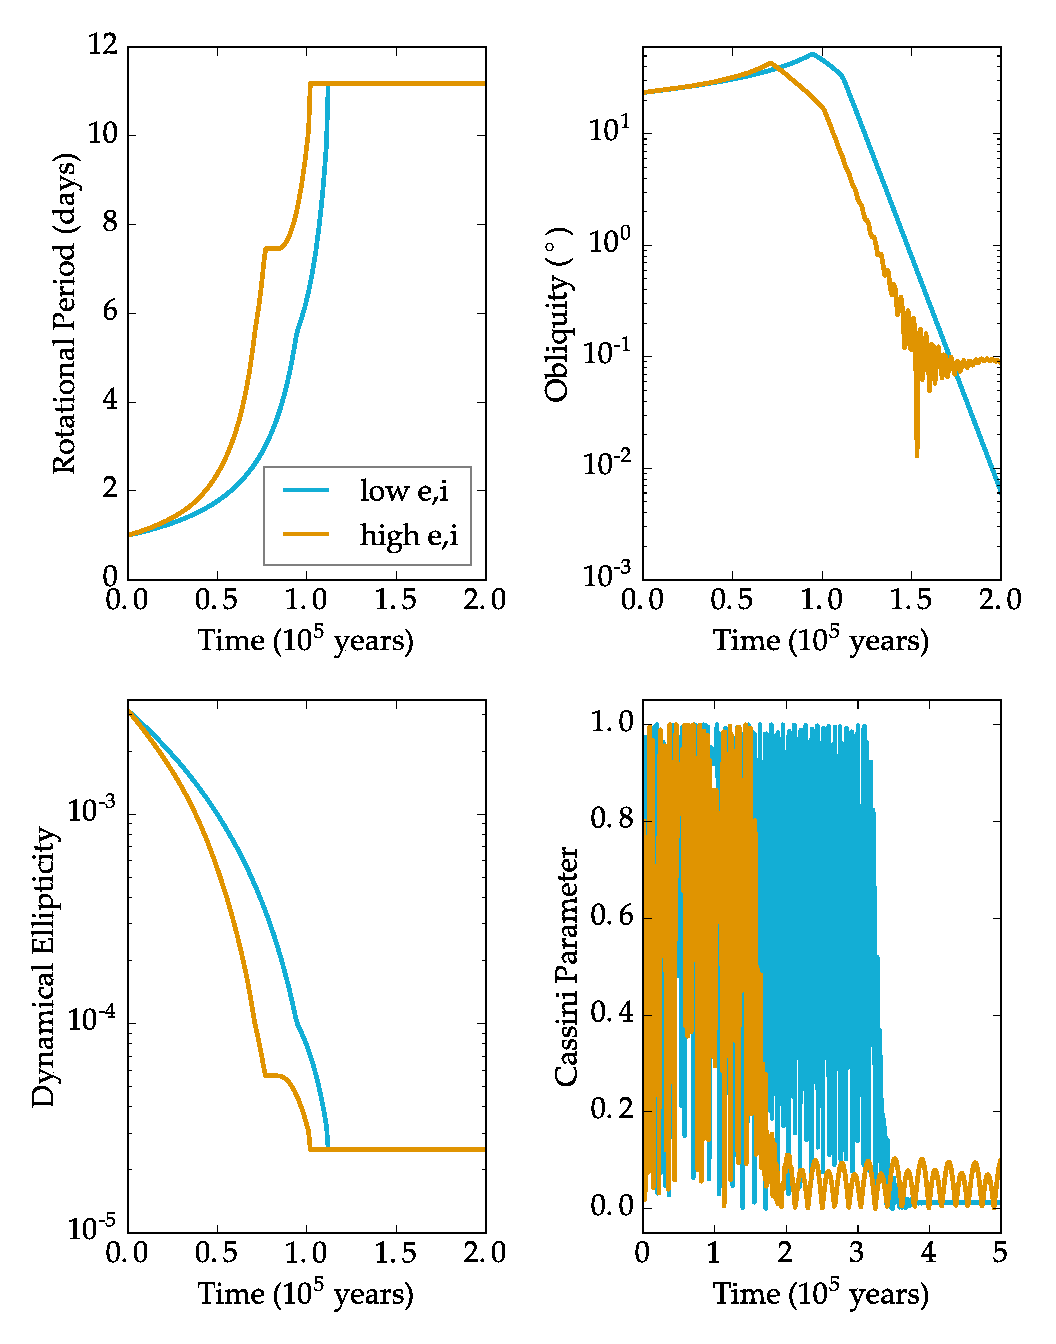
\includegraphics[width=0.75\textwidth]{MultiSpins2.eps}
\end{center}
\caption{Evolution of rotational properties of planet b for the two hypothetical multiplanet systems, with the low $e,i$ case in blue, and high $e,i$ case in orange. {\it Top left:} Rotation Period. {\it Top right:} Obliquity. {\it Bottom left:} Dynamical Ellipticity. {\it Bottom right:} Cassini Parameter.}
\label{fig:MultiSpins}
\end{figure}



% Fig 5: Low e/i case: a) Eccentricity, b) LongPeri, c) Inclination, d) LongNode
% Fig 6: High e/i case: a-d
% Fig 7: a) Rotation, b) obliquity for both cases

\subsection{Stellar Evolution}
\label{sec:results:stellar}
% Rodrigo

\xxx{Should Fig. 1 go here instead?}

In Fig.~\ref{fig:HZEvol} we plot the evolution of the conservative HZ
limits of \cite{Kopparapu13} as a function of time for a model of
Proxima Centauri; these are bounded by the runaway greenhouse limit
and the maximum greenhouse limit. The blue region is the HZ, which
slowly moves inwards for $\sim$ 1 Gyr, reaching the current orbit of
Proxima b after $\sim$ 160 Myr. In the atmospheric escape section
below, this is the value we assume for the duration of the runaway
greenhouse phase on Proxima b, during which water is allowed to
escape.

\begin{figure}[ht]
\centering
\includegraphics[width=5in]{HZEvol}
\caption{Evolution of the conservative HZ of Proxima Centauri, along with the orbits of Proxima Centauri b (solid line) and Mercury (dashed line).}
\label{fig:HZEvol}
\end{figure}

\subsection{Internal Evolution}
\label{sec:results:internal}
% Peter/Rory/Ben/David


The internal evolution of Proxima b is very difficult to model because
of the huge number of unknowns about its composition, initial
conditions, atmopshere, and the evolution of its environment, \eg
flares stripping the atmosphere. In this section we first consider how
different abundances of radiogenic isotopes could affect its
evolution, then we consider tidal heating.

%Fig 10: a) Tcore, b) Tman, c) RadPowerTot, d) SufEnFlux 
%       - one set with 26Al, one w/o

%Fig 10: a) Tcore, b) Tman, c) RadPowerTot, d) SufEnFlux 
%       - one set with 26Al, one w/o


As described in $\S$~\ref{sec:models:radheat} we consider four
possible abundance patterns for Proxima b: Earth-like, chondritic, 1
ppt $^{26}$Al, and inert. In all cases we begin with a core
temperature of 6000~K and a mantle temperature of 3000~K, except for
the chondritic case in which the latter is 4000~K. This change
was necessary to avoid discontinuities associated with the high
radiogenic power.

In Fig.~\ref{fig:radiog} we show the evolution of the radiogenic
power, mantle temperature, inner core radius, magnetic moment,
magnetopause radius and surface energy flux for the four cases. The
dashed black lines represent the modern Earth's value and all
intersect the Earth's curve (blue) at about 4.5~Gyr.

\begin{figure} 
\begin{center}
\includegraphics[width=0.75\textwidth]{NoTides.ps}
\end{center}
\caption{Evolution of internal properties of planet b for different
  assumptions of radiogenic inventory: Earth-like in blue, chondritic
  in orange, 1 part per trillion $^{26}$Al, and inert. Values for the
  modern Earth are shown with the dashed black line. {\it Top left:}
  Radiogenic power. The Earth curve is behind the $^{26}$Al curve for
  except for time = 0. {\it Top right:} Mantle Temperature. In the
  chondritic case (orange), the two kinks in the curve are due to the
  onset of core convection at 1.4~Gyr, and then due to the
  solidification of the mantle at 6.2~Gyr. Similarly the mantle
  solidifies in the $^{26}$Al (red) case at 2~Gyr. {\it Middle right:}
  Size of the solid inner core. {\it Middle left:} Magnetic
  moment. For the first 1.4 Gyr, the chondritic case has a
  non-convecting mantle and so it has no geodynamo. {\it Bottom left:}
  Magnetopause radius assuming the solar wind from Proxima is 0.2
  times that of Earth. {\it Bottom right:} Surface energy flux. The
  rapid variation in the chondritic case are associated with the onset
  of core convection, while the hump at 6 Gyr is due to the release of
  latent heat as the mantle solidies, as is the $^{26}$Al hump at 2
  Gyr.}
\label{fig:radiog}
\end{figure}

In the top left panel we show the evolution of the total radiogenic
power produced in the core, mantle and surface. Initially, the initial
power from $^{26}$Al is over $2 \times 10^{18}$~W, but with a
half-life of 700,000 years, its contribution to the energy budget
drops to 0 within $10^7$ years. The Earth-like case is hidden behind
the $^{26}$Al curve.

The mantle temperature is shown in the top right panel. The Earth and
inert cases are similar, but, as expected, the inert case temperature
drops more quickly becuase there is no radiogenic power in the
mantle. The enriched cases show interesting features as the energy
transport mechanisms change. The chondritic case shows two kinks, the
first is due to the onset of convection in the core, the second due to
heat production from the latent heat of solidification of the
mantle. Initially the heat generation from $^{40}$K is large enough to
heat the mantle to a temperature that is close enough to the core
temperature that convection is suppressed. The second kink occurs at
about 6~Gyr, or $\sim$6 half-lifes of $^{40}$K later. At that time, the
potassium power production has dropped sufficiently that the mantle
can begin to solidify and provides a new heat source. The $^{26}$Al
mantle solidifies at about 2~Gyr. Note that we had to start the
chondritic mantle at 4000~K, because at 3000~K, discontinuous heat
transfers developed since the mantle was so far from equilibrium
with the potassium power source.

The case with $^{26}$Al is particularly interesting because it
predicts initial mantle temperatures in excess of $10^4$~K, which is
hotter than the \xxx{surface of the} Sun. This result is clearly unphysical, and while some of the
issue is that we began this case with a mantle temperature of 3000~K,
the real problem is that the heating from just 1 ppt of $^{26}$Al is
so large that our model cannot handle it. However, we do see that
after this initial burst of heating, the planet calms down into an
Earth-like evolution. Thus, if heating from $^{26}$Al is just a
passing energy source, it may not affect the evolution. On the other
hand, the heating could be so large that the planet may be irrevocably
altered. At this time, we merely point out that the influence of
$^{26}$Al could be significant for planets with formation times of
order 1~Myr.

In the middle left panel, we show the size of the inner core. The
inert case produces the earliest inner core, but it does not consume the
entire core, which has a radius of 3400~km. The burst of $^{26}$Al
heating causing a slight delay in core formation compared to Earth,
while the chondritic case does not experience any core nucleation, even
after 7 Gyr.

The middle right panel shows the evolution of the magnetic moment of
Proxima b for the four different cases. The inert and Earth cases are
very similar, but the other two are very different. The $^{26}$Al case
has a very strong mangetic field early on, but it decays rapidly after
this power source is depleted. The chondritic case has no magnetic
field for the first 1.4 Gyr because the core/mantle temperature
difference is insufficient to generate convective motions in the
core. At that time, the core has cooled sufficiently to initiate
convection, and the geodynamo quickly grows to several times stronger
than the modern Earth.

The bottom left panel shows the magnetopause radius for Proxima
assuming a stellar wind that is 20\% weaker than the Sun's. This value
is an upper limit \citep{Wood01}, so our values here are conservative
-- the actual stand-off radius is larger -- except for the first
1.4~Gyr of the chondritic case for which there is no magnetic field.

Finally, the bottom right panel shows the surface energy flux for each
case. Not surprisingly the chondritic case maintains the highest heat
fluxes, near 1 W/m$^2$, which is similar to Io's value of 2.5
W/m$^2$~\citep{Veeder94}. The humps and kinks are due to the changing
heat sources described above. The $^{26}$Al case begins with a very
large heat flux, in the range of 100~W/m$^2$, which is nearing the
value to trigger a runaway greenhouse! The inert case emits less
energy than Earth. Note that this lower energy flux partially explains
the similarity in the mantle temperatures with time; the Earth case
produces and loses more energy than the inert case.

\subsubsection{Evolution with Tidal Heating}
\label{sec:results:internal:tides}

\xxx{atmesc results not described yet -- does this actually need to come later. I envisioned this subsection just being about themint/eqtide results. I'm not sure.}

Since a possible path towards habitability for Proxima b is the
``habitable evaporated core'' scenario of \citet{Luger15}, we seek to
model how the presence of an evaporating hydrogen envelope and surface
oceans impact the tidal and orbital evolution of Proxima b.  To do so,
we couple the atmospheric escape physics of \atmesc, tidal evolution
using \eqtide, the Earth-calibrated geophysical interior models of
\radheat \ and \thermint and the stellar evolution of \stellar.

We model the combined tidal contributions of the envelope, oceans, and solid interior via the following relation for the body's total tidal $Q$:
\begin{equation}
\label{eqn:Q_hec}
\frac{1}{Q} = \frac{1}{Q_{interior}} + \frac{1}{Q_{ocean}} +
\frac{1}{Q_{envelope}}
\end{equation}
where we remove $1/Q_i$ from the summation if we neglect the $i$th's
component contribution to Proxima b's net tidal interaction.  We
compute Proxima b's net 2nd Love number via
\begin{equation}
\label{eqn:k2_hec}
k_2 = k_{2_{interior}} + k_{2_{ocean}}+ k_{2_{envelope}}
\end{equation}
where again we remove $k_{2_{i}}$ from the summation if we neglect the
$i$th's component contribution to Proxima b's net tidal interaction.
In the general case when a hydrogen envelope is present, we only
consider the tidal effects of the interior and the envelope as any
water is likely to be super critical due to the high pressure exerted
by the envelope \xxx{(citation?)}.  When an envelope is not present,
we consider the tidal contribution of surface oceans if the planet is
not in the runaway greenhouse limit since all water would be present
in the atmosphere.

We simulate four reasonable boundary cases that bracket the potential
past tidal evolution of Proxima b.  The first case ``CPL'' assumes a
constant tidal $Q = 12$ analogous to the simulations seen in Figure
\ref{fig:eqtide}.  The ``No Ocean'' case assumes the tidal interaction
is dominated by the planet's interior as determined by \radheat \ and
\thermint while the ``Ocean" case which generalizes the No Ocean case
by assuming Proxima b had initially 10 Earth oceans of water with
$Q_{ocean} = 12$.  The full habitable evaporated core ``Envelope''
case generalizes Ocean by adding on a hydrogen envelope that has an
initial mass fraction of $0.001$ of the planet's total mass and
$Q_{envelope} = 10^4$ which is consistent with measurements of
Neptune's tidal Q \citep{ZhangHamilton08}.  The Envelope case also
starts with just 4.5 Earth oceans.  The results of the simulations are
shown in Figure \ref{tidal_hec}.

The No Ocean case, dominated by the mantle, reaches large tidal Qs
consistent with values reported by \cite{Zahnle15} for the early Earth
and undergoes minimal tidal evolution.  Radiogenic heating provides
most of the surface flux.  Early on, the Ocean case is in a runaway
greenhouse phase in which all the water is locked up in the atmosphere
and subject to escape of hydrogen and oxygen from photolysis,
decreasing the water mass.  Its tidal evolution mirrors the No Ocean
case as the mantle dominates.  Once the star's luminosity decreases
enough, the planet enters the HZ at around $10^8$ years and the
remaining water condenses to the surface. The presence of surface
oceans dramatically decreases the tidal Q leading to fast orbital
circularization and a massive surface flux increase via tidal energy
dissipation.

The Envelope case has an early bump in surface flux from rotational
tidal energy dissipation until the envelope has been completed removed
by stellar UV flux after about $4 \times 10^7$ years.  The hydrogen
envelope initially shielded the planet's water allowing for enough to
survive subsequent photolysis such that 1 Earth ocean of the initial
4.5 remained once the planet entered the HZ.  With the envelope gone,
surface water dominates the tides and its evolution mirrors that of
the Ocean case.

\xxx{A bit more to add once thermint+eqtide fully understood.}

% Fig 12: Same as 10, but with lines comparing oceanq, no ocean, CPL
\begin{figure} 
\centering
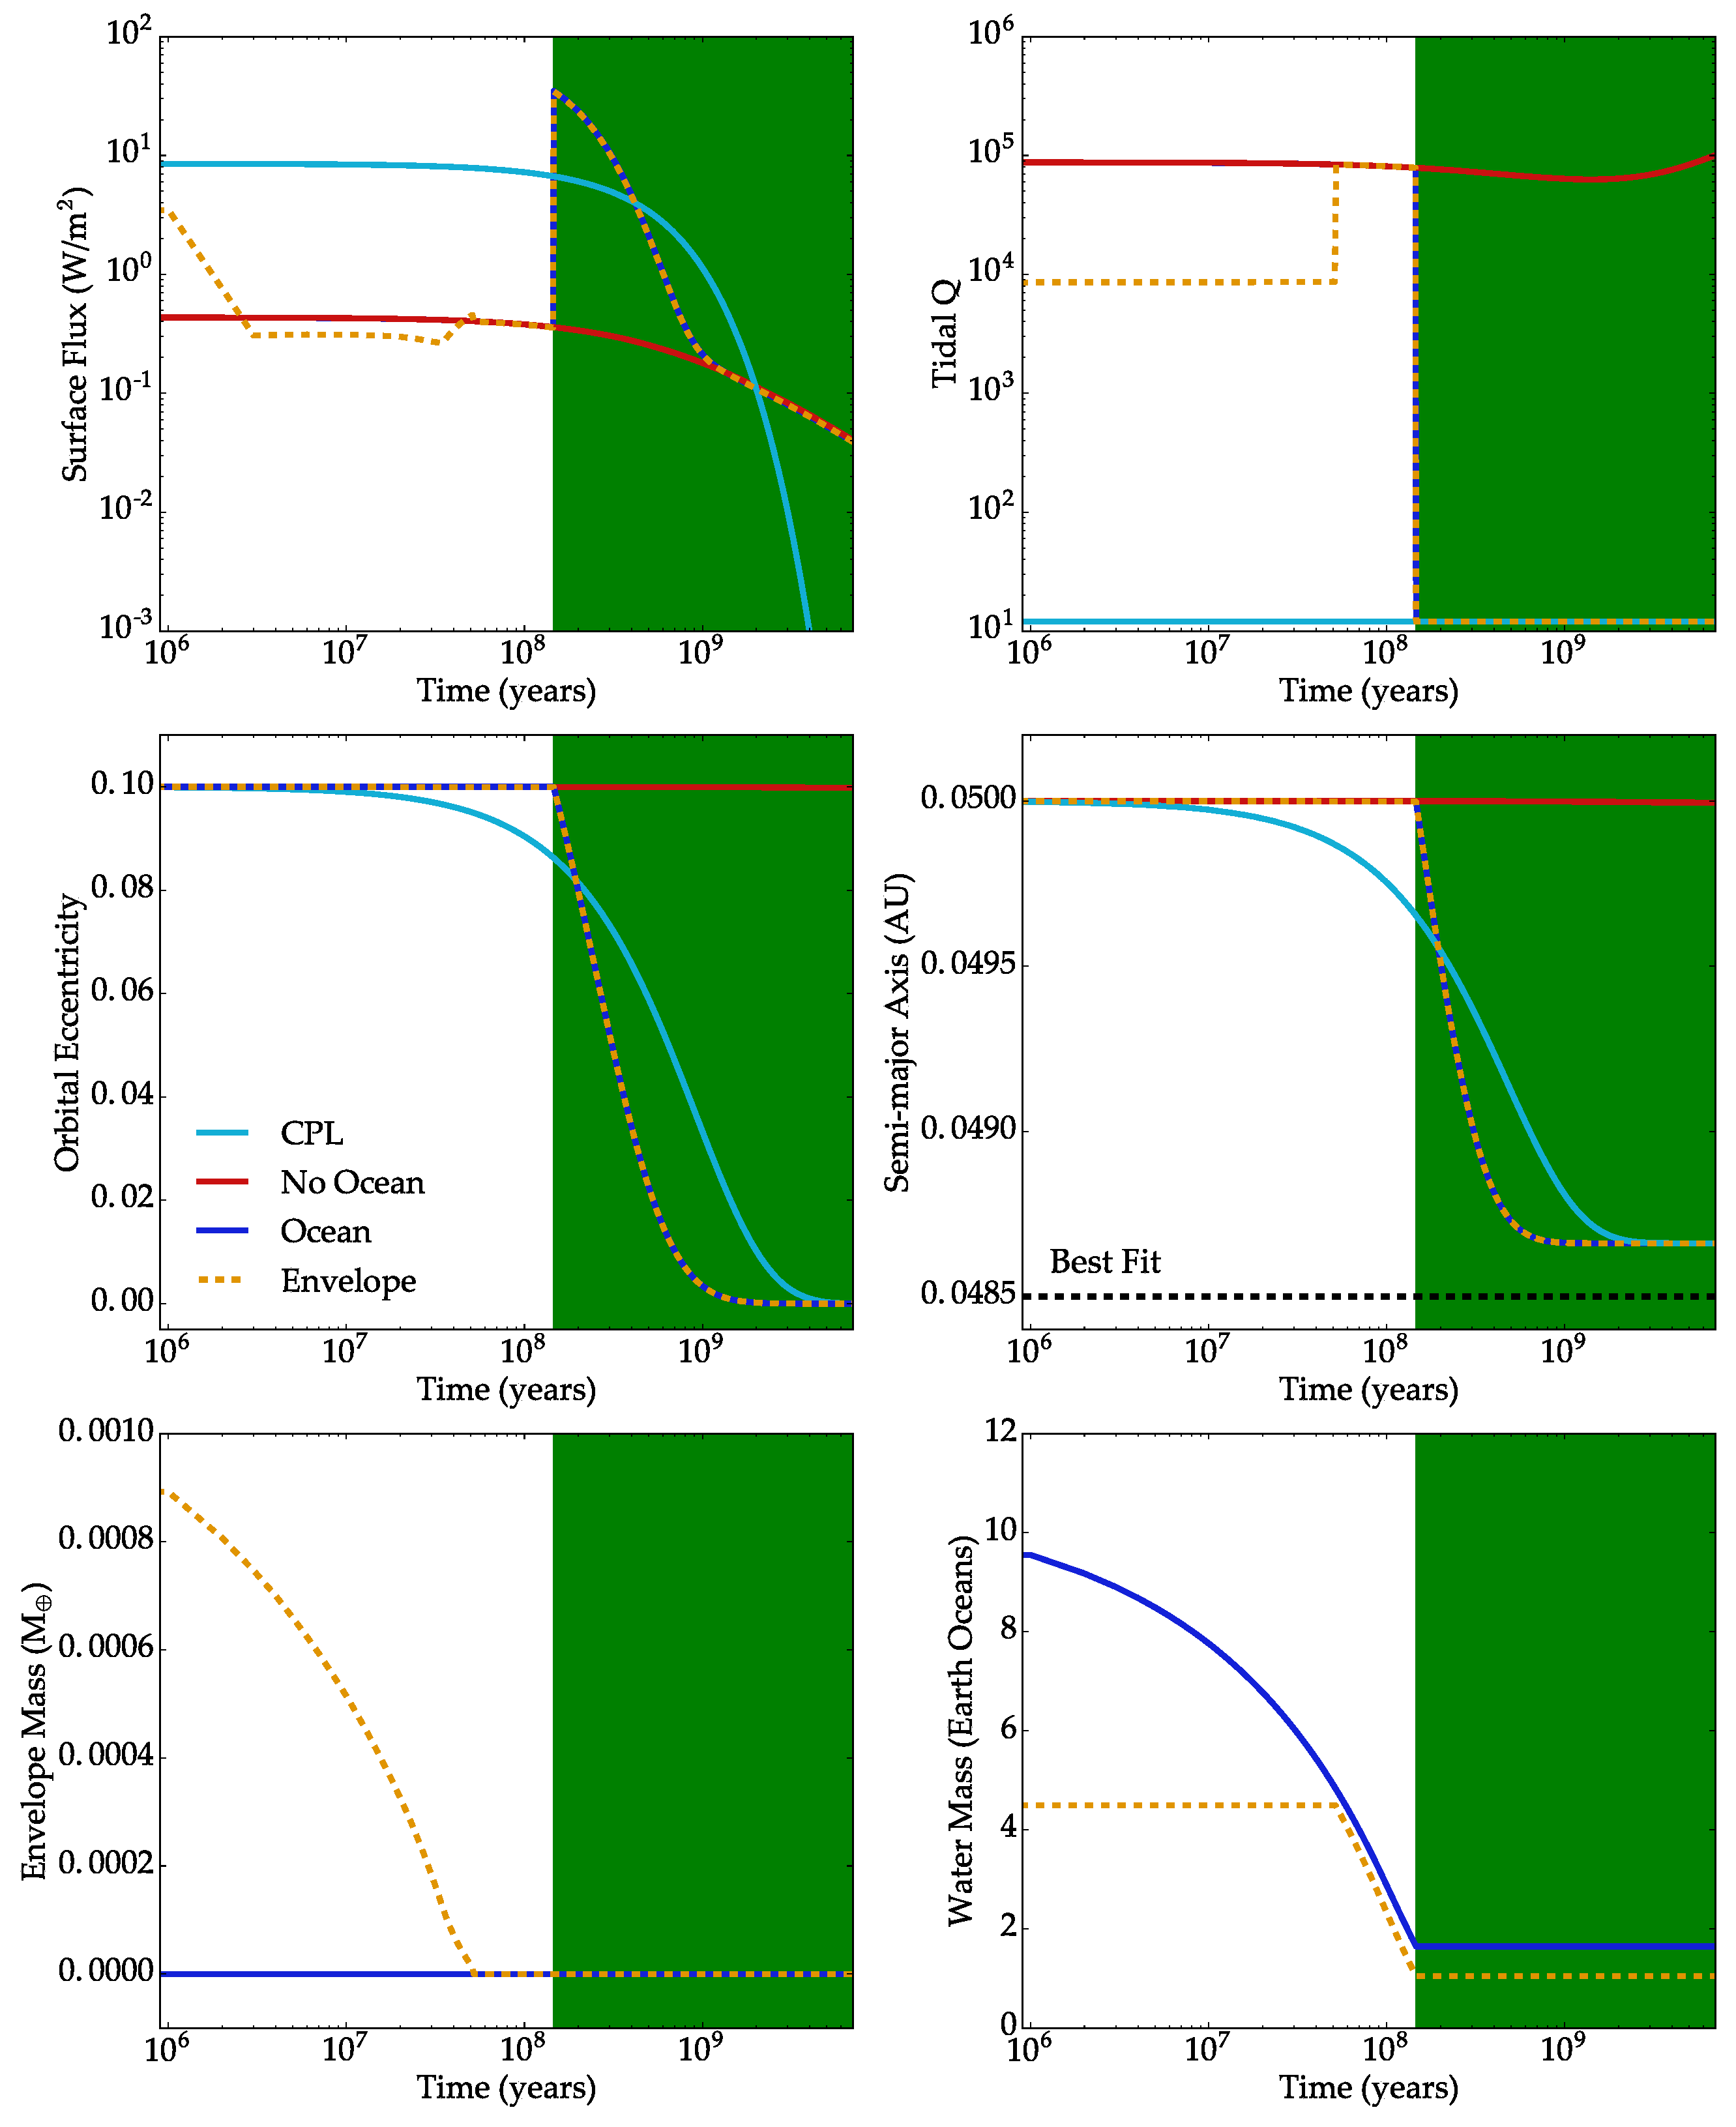
\includegraphics[width=1.0\textwidth,height=0.9\textheight]{tidal_hec.eps}
\caption{Evolution of the orbital, tidal and atmospheric properties of
  Proxima b for the ``CPL" case in light blue, ``No Ocean" case in
  red, ``Ocean" case in dark blue, and the ``Envelope" case in orange
  with the dashed line for clarity.  The green shaded region indicates
  when the planet is in the HZ. {\it Top left:} Surface Flux. {\it Top
    right:} Tidal Q. {\it Middle left:} Orbital Eccentricity. {\it
    Middle right:} Semi-major Axis. {\it Bottom left:} Envelope
  Mass. {\it Bottom right:} Surface Water Mass. \xxx{I don't like the red on green.} 
  \xxx{rd: can I suggest replacing the green with a light gray? or a single vertical 
  dashed line?} }
\label{fig:tidal_hec}
\end{figure}

% Fig 13: a) MagMom, b) WindPres, c) MagRad
%       - one set of curves w/tidal heat, one w/o

\subsection{Atmospheric Evolution}
\label{sec:results:atmesc}
% Rodrigo

In Fig.~\ref{fig:HZEvol} we plot the evolution of the conservative HZ limits of \cite{Kopparapu13} as a function of time for a model of Proxima Centauri. The blue region is the HZ, which slowly moves inwards for 500 Myr, reaching the current orbit of Proxima b after about 200 Myr.

\begin{figure}[ht]
\centering
\includegraphics[width=6in]{mirage}
\caption{Evolution of the water content and atmospheric O$_2$ pressure
  on Proxima b for different initial conditions. The initial water
  content is varied between 1 and 10 TO (various colors) for two
  different end-member scenarios: no O$_2$ surface sinks (solid lines)
  and instantaneous oxygen absorption at the surface (dashed
  lines). The planet mass is held constant at 1.27 M$_\oplus$ and the
  initial hydrogen envelope fraction is set to zero for all runs. In
  all but one of the runs, Proxima b is completely desiccated. For an
  initial water content of 10 TO and no surface sinks, the buildup of
  $\sim$ 500 bars of atmospheric O$_2$ slows the loss rate of H,
  preventing the last $\sim$ 1 TO of water from being lost. In the
  scenario that efficient oxygen sinks are present, the atmospheric
  O$_2$ mixing ratio never grows sufficiently to limit the escape of
  H, and desiccation occurs in all cases. Note that in this scenario,
  the curves in the ``O$_2$ pressure'' panel correspond to the
  equivalent O$_2$ pressure absorbed at the surface.}
\label{fig:atmesc:mirage}
\end{figure}

In Fig.~\ref{fig:atmesc:mirage} we show the evolution of the latter
type of planet, which formed with no significant primordial
envelope. We consider four different initial inventories of water: 1,
3, 5, and 10 terrestrial oceans (1 TO $\equiv 1.39\times 10^{24}$ g,
the total mass of surface water on Earth; see \cite{Kasting88}). As
discussed in $\S$~\ref{sec:models:atmesc}, we also consider two end-member
scenarios regarding the photolytically-produced O$_2$: no surface
sinks (solid lines) and efficient surface sinks (dashed lines). In all
cases but one, the planet is completely desiccated within the first
160 Myr, building up between tens and hundreds of bars of O$_2$ in
either its atmosphere or in the solid body. For an initial water
content of 10 TO and no surface sinks, O$_2$ builds up to high enough
levels to throttle the supply of H to the upper atmosphere and slow
the total escape rate. In this scenario, $\sim 1$ TO of water remains,
alongside a thick 500 bar O$_2$ atmosphere. If Proxima b formed with
less than ten times Earth's water content, and/or had a persistent
convecting, reducing magma ocean, it is likely desiccated today.

\begin{figure}[ht]
\centering
\includegraphics[width=6in]{hec}
\caption{Evolution of the water and O$_2$ contents assuming Proxima b
  formed with a hydrogen envelope and 3 TO. Line colors correspond to
  different initial envelope mass fractions $f_H$, ranging from 0.0001
  to 0.01. In all cases, the envelope evaporates completely prior to 1
  Gyr. For $f_H \lesssim 0.001$, the H envelope evaporates quickly
  enough to allow complete desiccation of the planet prior to its
  arrival in the HZ at $\sim$ 160 Myr. For $f_H \approx 0.01$, the
  envelope evaporates a few hundred Myr \emph{after} the planet enters
  the HZ, preventing any water from being lost and O$_2$ from
  accumulating in the atmosphere.  This is the most favorable scenario
  for a potentially habitable Proxima b.}
\label{fig:atmesc:hec}
\end{figure}

Next, in Fig.~\ref{fig:atmesc:hec}, we show the results assuming
Proxima b formed with a hydrogen envelope. We fix the initial water
content at 3 TO and consider initial envelope mass fractions $f_H$
ranging from $10^{-4}$ to $10^{-2}$. In all cases, the envelope
evaporates completely within the first several hundred Myr. For $f_H
\lesssim 10^{-3}$, the envelope evaporates early enough such that all
the water is still lost from the planet. For $f_H = 10^{-3}$, only
about 0.1 TO remain once the planet enters the HZ; only for $f_H \sim
10^{-2}$ does the presence of the envelope guard against all water
loss. In these calculations, we assumed inefficient surface sinks, so
the escape of water at late times was bottlenecked by the presence of
abundant O$_2$. Planets that form with hydrogen envelopes may have
quite reducing surfaces, which could absorb most of the O$_2$ and lead
to even higher total water loss. As before, a few tens to a few
hundreds of bars of O$_2$ remain in the atmosphere or in the solid
body at the end of the escape phase.

We note that we obtain slightly more hydrogen loss than
\cite{OwenMohanty16}, who find that planets more massive than $\sim
0.9 \mearth$ with $\sim 1\%$ hydrogen envelopes cannot fully lose
their envelopes around M dwarfs, due primarily to the transition from
hydrodynamic to ballistic escape at late times. However, their
calculations were performed for a $0.4 \msun$ M dwarf, whose pre-main
sequence phase lasts $\sim 200 \mathrm{Myr}$, five times shorter than
that for Proxima Centauri. Nevertheless, the discrepancy is small: we
find that for envelope fractions greater than 1\% or masses greater
than our fiducial value of $1.27 \mearth$, the envelope does not
completely evaporate, in which case Proxima b would likely be
uninhabitable.

\begin{sidewaysfigure}[h]
\centering
\subfigure{\label{fig:atmesc:synth:a}\imagebox{2.5in}{\includegraphics[width=3.3in]{synth_a}}}
\subfigure{\label{fig:atmesc:synth:b}\imagebox{2.5in}{\includegraphics[width=3.3in]{synth_b}}}
\subfigure{\label{fig:atmesc:synth:c}\imagebox{2.5in}{\includegraphics[width=1.285in]{synth_c}}}
\caption{Multiple evolutionary pathways for the water on Proxima
  b. These plots show the final water and final O$_2$ content of the
  planet for a suite of different initial conditions. Different marker
  styles indicate different values of the planet mass, the initial
  water content, and the initial hydrogen envelope mass fraction $f_H$
  (the final value of $f_H$ is zero for all planets shown here).  The
  left panel corresponds to planets with inefficient O$_2$ sinks,
  which build up O$_2$ in their atmospheres during the hydrodynamic
  escape phase. The right panel corresponds to planets with efficient
  sinks, which do not build up significant atmospheric O$_2$; instead,
  O$_2$ is quickly absorbed at the surface. Each panel is divided into
  quadrants, corresponding to planets that at the end of the
  simulation have water but no O$_2$ (top left), water and O$_2$ (top
  right), neither water nor O$_2$ (bottom left), and O$_2$ but no
  water (bottom right). Habitable planets are those in regions shaded
  blue. Planets in the grey region are desiccated and therefore
  uninhabitable. Planets in the red regions are likewise
  uninhabitable, but may have atmospheric O$_2$ (left panel only)
  which could be incorrectly attributed to biology. Finally, planets
  in the yellow region are habitable, since they have abundant surface
  water, but may also have substantial atmospheric O$_2$, which could
  be an impediment to the origin of life. These planets are also
  particularly problematic in the context of atmospheric
  characterization, as the presence of water and O$_2$ could fool
  observers into believing they are inhabited.}
\label{fig:atmesc:synth}
\end{sidewaysfigure}

Finally, in Fig.~\ref{fig:atmesc:synth} we present a summary of our
atmospheric escape calculations, showing the many possible
evolutionary pathways for Proxima b and how they affect its present
habitability. The two panels show the final water content (in TO)
versus the final oxygen abundance (in bars) for different initial
conditions, assuming inefficient oxygen sinks (left panel) and
efficient oxygen sinks (right panel). In all cases shown, the final
hydrogen envelope mass is zero.  Different values of the planet mass,
initial water content, and hydrogen fraction are indicated with
different marker styles (see legend at right). Since the axes are
logarithmic, we appended panels to the left and below the main plot,
corresponding respectively to final oxygen and water contents of
zero. In general, habitable outcomes are those that lie in the top
left of the plot (abundant water, low O$_2$). Planets in the top right
have abundant water but also build up large amounts of O$_2$, which
could render them uninhabitable and/or fool
observers searching for biosignatures \citep{LugerBarnes15}. Planets at the bottom of the
plot are desiccated and therefore uninhabitable, though some may also
be biosignature false positives.

While much may be gleaned from the figure, a few results stand
out. First, a scenario in which Proxima b formed with a hydrogen
envelope of mass $\sim 0.01 \mearth$ is the most favorable for
habitability, as such a planet would be a ``habitable evaporated
core'' \citep{Luger15} and experience no water loss. However, if
Proxima b is more massive than $1.27 \mearth$, the envelope may not
completely evaporate and the planet may not be habitable
today. Second, scenarios in which Proxima b formed with less hydrogen
can still result in present-day surface water, but in all cases in
which water remains, $\gtrsim 200$ bars of oxygen are
retained. Finally, the primary effect of a larger planet mass is to
increase the amount of oxygen in the atmosphere and/or absorbed at the
surface; while in some cases a larger planet mass can result in less
water loss, habitable scenarios are more likely for a lower planet
mass, consistent with the results of \cite{LugerBarnes15}.

Further data on Proxima b will greatly aid in distinguishing between
these multiple evolutionary pathways. In particular, constraints on
the exact mass (via measurements of the orbital inclination) could
inform the atmospheric escape history, while a value for the radius
could provide a handle on whether or not a hydrogen envelope is
present.

\section{Discussion\label{sec:disc}}
% All

In the previous section we outlined numerous possibilities for the
history of Proxima b. We considered processes spanning the planet's
core to the Milky Way galaxy and find that effects at all these scales
could be important in the history of our closest exoplanet. In this
section, we summarize the results in terms of the potential
atmospheres that Proxima b might have, which are considered in
detail in \citep{Meadows16}. Then we examine the likelihood that it is
currently habitable.

\subsection{Atmospheric States}
\label{sec:results:atmstates}

\xxx{dflemin3:  In this subsection, I think it could be useful to tie by in the concept of abiotic spectral features that can 
masquerade as biosignatures.  For example, in the Abiotic section, Luger-Barnes O2 build up can be a tricky thing to
disentangle from life-produced oxygen.  Obviously the companion atmosphere paper deals with all these effects in much
better detail, but since this issue was mentioned as a problem in the intro, briefly touching on it again here would be useful.}

\subsubsection{Earth-Like}
\label{sec:results:atmstates:earthlike}

We find that some scenarios allow for the planet to currently support liquid
surface water. In particular, the ``habitable evaporated core'' scenario
\citep{Luger15} is particularly promising as it can avoid both the
high-luminosity pre-MS phase and any devastating tidal
heating that may occur while the planet ``surfs'' the HZ migration, or
during circularization after orbital destabilization. Such a world may
be enriched in deuterium that remained during \xxx{hydrogen} escape, and it
may also be geothermally active if it is young and enriched in
potassium.

Another possibility is that Proxima b formed at a larger orbital
distance and was scattered in to its current location by a system-wide
instability, which may have been triggered by a close passage with
\acen~A and B, see $\S$~\ref{sec:results:galactic}. If the instability
happened after the star reached the main sequence, then the planet
would have arrived in the HZ after its position had stabilized. If b's
eccentricity after the instability was larger than about 0.35, then
there is some danger that tidal heating could have triggered a runaway
greenhouse, \xxx{see Fig.~\ref{fig:eqtide}}, but it may have been
short-lived enough to permit habitability.

Another low-probability possibility is that even if the planet became
desiccated during the pre-MS phase, impact from water-rich bodies
could simultaneously blow off the CO$_2$ and/or O$_2$ atmosphere while
delivering water. This scenario would require a specific set of events to occur, but we note
that close passages between Proxima and \acen~A and B could destabilize
any putative ``exo-Oort Clouds'' that could have existed around the
stars. Current numerical models do not permit a robust calculation of
this possibility, so it remains a viable path for Proxima b to be
habitable. \xxx{REF for exo-Oort clouds?} \xxx{rd: not sure a reference is 
necessary here. We are just speculating that since the sun
has an Oort cloud, it is possible for other stars to have them (Copernican
principle). I'm not sure a good reference even exists.}

Although these atmospheric states permit habitability, we must bear in
mind that the rotation period is either synchronous or in a spin-orbit
resonance due to tidal effects. The rotation rate is therefore longer
than on Earth and so atmospheric dynamics would be different. If
synchronous, it is likely that the planet's daylit side is
covered in clouds \citep{Yang13}.

\subsubsection{Venus-Like}
\label{sec:results:atmstates:venuslike}


Regardless of whether Proxima b spent significant time in a runaway
greenhouse prior to the arrival of the HZ, it could be in a runaway
greenhouse state like Venus. If it formed {\it in situ}, then this
possibility is more likely because its first $\sim$100 Myr were spent
interior to the HZ and hence it may have developed a dense CO$_2$
atmosphere as has occurred on Venus. In this case, the planet is
uninhabitable as the surface temperature is too hot for liquid water,
and the higher surface temperature results from greenhouse warming by
CO$_2$.

Even if the planet avoided desiccation during the Pre-MS stage, it is
reasonable to assume that a Venus-like atmosphere is possible. CO$_2$
is a very abundant molecule in planetary atmospheres, and given its
strong ability to heat \xxx{the} surface, high molecular weight, and strong
chemical bonds, it may be able to accumulate in the HZ to large enough
levels to trigger the runaway greenhouse. \xxx{[Colin Goldblatt's
paper actually shows that adding CO2 alone cannot cause a runaway
greenhouse on an Earth-like planet: http://arxiv.org/abs/1201.1593.
I don't disagree with the possibility that it's in a runaway even in 
the HZ, but perhaps a better argument is if its albedo is < 0.3 or if
clouds behave differently, etc.?] -- RB: I thought that paper was about burning through all the fossil fuels on Earth.}

A final possibility, mentioned above, is that past tidal heating drove
the planet into a runaway greenhouse \citep{Barnes13}. If the planet
was ever in a high eccentricity state ($e~>~0.35$) then the surface
energy flux from the interior could have reached the critical limit of
$\sim$300 W/m$^2$ \citep{Kasting93,Abe93,Goldblatt15}. Such high
surface fluxes may be short-lived if the heating can only come from
the ocean \citep{DriscollBarnes15}.

\subsubsection{Neptune-Like}
\label{sec:results:atmstates:neptunelike}

Proxima b may have formed with sufficient hydrogen that some has been
retained despite all the high energy processes that can remove
it. This possibility is especially likely if it formed beyond the snow
line and migrated in. Similarly to \cite{OwenMohanty16}, we find that
if Proxima b formed with $\gtrsim$ 1\% of its mass in the form of a
hydrogen envelope, it could still possesses some hydrogen, in which
case the surface may be too hot and/or the surface pressure is too
high for habitability.  Future measurements of Proxima b's radius can
inform its present-day composition and thus settle this issue.
% rodluger: Removed ``perhaps with 10 times more mass than it has now'',
% as that's not really physical. At most it's lost about 1\% H/He.

\subsubsection{Abiotic Oxygen Atmosphere}
\label{sec:results:atmstates:o2atmos}

If Proxima b formed with one or more TO of water, photolysis followed
by hydrogen escape during the stellar Pre-MS phase could have led to the 
buildup of substantial O$_2$ in the atmosphere. Although oxygen
is highly reactive, thousands of bars of oxygen can be liberated
through this mechanism \citep{LugerBarnes15} and hence all sinks for
it may become saturated \citep{Schaefer16}. In principle, thousands of
bars of oxygen could remain in the atmosphere, but this figure is most likely lower,
as much of the oxygen will be consumed in the process of oxidizing the surface. 
In this case Proxima b may be uninhabitable, given that little free energy
may be available at the surface for early organisms to take a hold. Life on
Earth is thought to have emerged in an extremely reducing environment
\citep{Oparin24, Haldane29}, with access to high energy gradients to fuel
early metabolisms; this may not be the case on Proxima b.

In many of the scenarios in which Proxima b develops an O$_2$-rich atmosphere,
it also maintains at least some of its initial water.
After the end of the Pre-MS phase, the O$_2$, H$_2$O and CO$_2$
greenhouse warming could be sufficient to prevent water from
accumulating on the surface, and hence it could have significant
abundance in the stratosphere. While the simultaneous detection of
water and oxygen has traditionally been envisaged as an ideal
combination for life detection (\xxx{REF}), in the case of Proxima b, it is
insufficient to prove habitable conditions exist, let alone that life
is present.

Alternatively, if the greenhouse gases are at low enough levels in the atmosphere,
then it may be possible for liquid water to accumulate on the
planetary surface and this planet would meet the traditional
definition of ``habitable.'' However, as argued above, such a planet
would likely be incapable of supporting life.
Thus, the detection of atmospheric oxygen as well as the
presence of surface liquid by other means, \eg glint
\citep{Robinson10}, would not be sufficient evidence that the planet
is habitable.

\subsubsection{No Atmosphere}
\label{sec:results:atmstates:noatmos}

Since Proxima b is subjected to repeated flaring events and other
activity \citep{Walker81,Davenport16}, it may be that the
atmosphere has been \xxx{permanently} destroyed. Such a process is
difficult to envision, as it would require all the volatiles in the
mantle to have been degassed and blown away. However, if the planet
was tidally heated for a long time, mantle convection may have been
vigorous and perhaps total volatile depletion is possible, especially
if the planet is of order 7 Gyr old and if the core has \xxx{solidified},
quenching the magnetic dynamo \xxx{\citep{DiscollBarnes15}}. Another possibility is that a recent
stellar eruption has temporarily stripped away the atmosphere, which
will reform by outgassing.

\xxx{Other possibilities? It could be dry because 26Al heating prevented accumulation of hydrated silicates. Abe found incident fluxes $< 415$W/m2 were not in runaway. We want a comprehensive list here.}


\subsection{Is Proxima b Habitable?}
\label{sec:results:habitable}

Planetary habitability is a complicated feature to model
quantitatively and Proxima b is no exception. We do know that the
planet has sufficient energy to support life, assuredly has enough
bioessential elements, and is old enough for life to have gained a
foothold, assuming Earth isn't an extreme outlier. The biggest
questions are if it is terrestrial, and if it possesses vast \xxx{reservoirs}
of liquid water. At this time, it is impossible to determine the
probability that it does support liquid water, so we cannot answer the
eponymous question. As always, more data are needed.

However, our analysis does provide some important information on where
to focus future efforts. As liquid water is vital, it is paramount to
determine the pathways that allow the planet to have accreted and
retained the water. However, even if the planet forms with water, our
investigations have shown that it will not necessarily be retained. If
it formed {\it in situ} or arrived in the HZ at the time of the
dispersal of the gas disk, then Proxima b had to endure $\sim$ 150
Myr in a runaway greenhouse state; see $\S$~\ref{sec:results:stellar} and
\cite{LugerBarnes15}.

Even if the planet arrived in its orbit late, perhaps following an
orbital instability, the water may have to survive a ``tidal
greenhouse'' in which tidal heating drives water loss, see
$\S$~\ref{sec:results:internal}. and \citep{Barnes13}. Such high tidal heating
rates may require very large eccentricity and/or abnormally low $Q$
values, but the former is certainly possible during planet-planet
scattering events \citep{Chatterjee08}, or perhaps by Kozai-like
oscillation driven by perturbations from the \acen~A and B pair if the
orbit of Proxima Centauri was much smaller in the past
\citep{DesideraBarbieri07}. If the additional planet in the system is
massive, on an eccentric orbit, and/or on a highly inclined orbit,
then it, too, may induce eccentricity perturbations that maintain
eccentricities \citep{TakedaRasio05}, possibly in the range of a tidal
greenhouse. As shown in $\S$~\ref{sec:results:internal}, the eccentricity of
b will damp, but the timescale can be very long. Large eccentricities
are not well-modeled by equilibrium tide theory, even with a proper
accounting of geophysical features as in the \thermint module, so it
is difficult at present to assess the role of tidal heating in water
retention.

Another possible route to water loss is through temporary or permanent
atmosphere erosion by flares and coronal mass ejections. It is
possible that these events could blast away the atmosphere completely,
in which case liquid water on the surface is not stable. Should the
atmosphere reform, the water may return to the liquid state, but it is
certainly plausible that some events are powerful enough to remove the
water in one event, or, more likely, repeated bombardments would
slowly remove the \xxx{atmosphere}. \xxx{REF: Matt Tilley paper or Segura?} Our analysis doesn't provide a direct
measurement of this phenomenon, but we note that some geophysical
models for the planet predict core solidification times less than the
age of the system \xxx{which models?}. In those cases, the magnetic field is quenched and
is not capable of deflecting charged particles. However, it is not
clear that a magnetic field is always beneficial for life, as it also
increases the cross-sectional area of the planet for charged particles
and funnels the energy into the magnetic poles, possibly increasing
mass loss.

These processes are all clear dangers for the habitability of Proxima
b. Yet, we are also able to identify pathways that produce decidedly
Earth-like versions of planet b. \xxx{As shown in Fig.~\ref{fig:qchoice},
if the planet formed with 0.1\% of its mass in a hydrogen envelope, 4.5
Earth oceans of water, then the combined effects of the stellar
evolution, envelope evolution and atmospheric escape, tidal evolution,
and geophysical evolution predict a planet with 1 Earth ocean of
surface water, no hydrogen envelope, and a semi-major axis within the
observed uncertainties [Dave: Check these numbers]}. A planet like this could evolve similarly to
Earth, and therefore may have Earth-like conditions today.

A final possibility is that Proxima b, receiving only 65\% of Earth's
insolation, may have an ice-covered surface, but with a liquid water
mantle, similar to Europa. For such a planet, the water is heated by
the energy from accretion, radiogenic sources and/or tidal
heating. Ice is much more absorptive at the longer wavelengths of
light that Proxima emits and so it may be difficult to ice over the
planet \xxx{\citep{Joshi12,Shields13}}, especially since it probably spent
hundreds of Myr in a runaway greenhouse. But if a reflective haze
and/or cloud layer could form, it could reflect away the light before
it reaches the surface \xxx{REF: Giada citation?}. This possibility seems unlikely, but we cannot
rule out that the planet is a ``super-Europa'' \citep{BarnesHeller13},
a scaled up version of the icy satellites of our Solar System and with
a potentially inhabited subsurface water layer.

Proxima b may or may not be habitable. While we are only able to
identify a narrow range of pathways that permit habitability, we must
bear in mind that our model, while including phenomena over sizescales
of meters to kpc, is simple and does not include many potential
feedbacks. The geochemistry of exoplanets is a gaping hole in
scientific knowledge, and one can easily imagine how other systems may
maintain liquid water with geochemical cycles not present in our Solar
System. Similarly, liquid surface water may represent a sort of
``planetary attractor,'' in which planets in the HZ naturally and
typically evolve toward a state in which their surfaces support liquid
water. 

\section{Conclusions\label{sec:concl}}
% Rory
We have performed a comprehensive analysis of the evolution of the
Alpha Centauri triple star system with a specific focus on Proxima Centauri b's
habitability. We find that many disparate factors are important,
including the stellar system's orbit in the galaxy
($\S$~\ref{sec:results:galactic}), the orbital and rotational evolution of
the planets ($\S$~\ref{sec:results:orbital}), the stellar evolution
($\S$~\ref{sec:results:stellar}), the geophysical evolution
($\S$~\ref{sec:results:internal}), and the atmospheric evolution
($\S$~\ref{sec:results:atmesc}). We find that many evolutionary pathways
are admitted by the data and hence the planet may currently exist in
one of many possible states.

We conclude that Proxima b may be habitable, but identify the
retention of water as the biggest obstacle for Proxima b to support
life. Water loss may occur through multiple channels operating in
tandem or in isolation, including desiccation during the Pre-MS,
excessive tidal heating, or atmospheric destruction by flares and
coronal mass ejections. We find the most likely pathway for
habitability is if planet b formed with a thin hydrogen envelope of
order $10^{-2}~\mearth$ which was eroded by the early XUV evolution of
the host star; see $\S$~\ref{sec:results:stellar} and \cite{Luger15}. In
that case, Proxima b is a ``habitable evaporated core'' and has
followed a very different trajectory than Earth did on their paths to
liquid surface water.

Regardless of Proxima's habitability, it offers scientists an
\xxx{unprecedented} window into the nature of terrestrial planets. At only
1.3 pc distance, we will be able to study this planet in detail with
future missions, should they be designed appropriately; see
\cite{Meadows16}. If Proxima b is uninhabitable, we may be able to
determine how that happened and how Earth avoided the same fate. At a
minimum, the discovery of Proxima Centauri b has ushered in a new era
in comparative planetology, or perhaps it is the first step in the
discovery of extraterrestrial life.
 
\vspace{1cm}
This work was supported by the NASA Astrobiology Institute's Virtual
Planetary Laboratory under Cooperative Agreement number NNA13AA93A.
David Fleming is supported by an NSF IGERT DGE-1258485 fellowship.


\bibliography{bib}

\end{document}  
